% Options for packages loaded elsewhere
\PassOptionsToPackage{unicode}{hyperref}
\PassOptionsToPackage{hyphens}{url}
%
\documentclass[
]{book}
\title{Rmarkdown and Shiny}
\author{Lei mingri}
\date{2021-12-13}

\usepackage{amsmath,amssymb}
\usepackage{lmodern}
\usepackage{iftex}
\ifPDFTeX
  \usepackage[T1]{fontenc}
  \usepackage[utf8]{inputenc}
  \usepackage{textcomp} % provide euro and other symbols
\else % if luatex or xetex
  \usepackage{unicode-math}
  \defaultfontfeatures{Scale=MatchLowercase}
  \defaultfontfeatures[\rmfamily]{Ligatures=TeX,Scale=1}
\fi
% Use upquote if available, for straight quotes in verbatim environments
\IfFileExists{upquote.sty}{\usepackage{upquote}}{}
\IfFileExists{microtype.sty}{% use microtype if available
  \usepackage[]{microtype}
  \UseMicrotypeSet[protrusion]{basicmath} % disable protrusion for tt fonts
}{}
\makeatletter
\@ifundefined{KOMAClassName}{% if non-KOMA class
  \IfFileExists{parskip.sty}{%
    \usepackage{parskip}
  }{% else
    \setlength{\parindent}{0pt}
    \setlength{\parskip}{6pt plus 2pt minus 1pt}}
}{% if KOMA class
  \KOMAoptions{parskip=half}}
\makeatother
\usepackage{xcolor}
\IfFileExists{xurl.sty}{\usepackage{xurl}}{} % add URL line breaks if available
\IfFileExists{bookmark.sty}{\usepackage{bookmark}}{\usepackage{hyperref}}
\hypersetup{
  pdftitle={Rmarkdown and Shiny},
  pdfauthor={Lei mingri},
  hidelinks,
  pdfcreator={LaTeX via pandoc}}
\urlstyle{same} % disable monospaced font for URLs
\usepackage{color}
\usepackage{fancyvrb}
\newcommand{\VerbBar}{|}
\newcommand{\VERB}{\Verb[commandchars=\\\{\}]}
\DefineVerbatimEnvironment{Highlighting}{Verbatim}{commandchars=\\\{\}}
% Add ',fontsize=\small' for more characters per line
\usepackage{framed}
\definecolor{shadecolor}{RGB}{248,248,248}
\newenvironment{Shaded}{\begin{snugshade}}{\end{snugshade}}
\newcommand{\AlertTok}[1]{\textcolor[rgb]{0.94,0.16,0.16}{#1}}
\newcommand{\AnnotationTok}[1]{\textcolor[rgb]{0.56,0.35,0.01}{\textbf{\textit{#1}}}}
\newcommand{\AttributeTok}[1]{\textcolor[rgb]{0.77,0.63,0.00}{#1}}
\newcommand{\BaseNTok}[1]{\textcolor[rgb]{0.00,0.00,0.81}{#1}}
\newcommand{\BuiltInTok}[1]{#1}
\newcommand{\CharTok}[1]{\textcolor[rgb]{0.31,0.60,0.02}{#1}}
\newcommand{\CommentTok}[1]{\textcolor[rgb]{0.56,0.35,0.01}{\textit{#1}}}
\newcommand{\CommentVarTok}[1]{\textcolor[rgb]{0.56,0.35,0.01}{\textbf{\textit{#1}}}}
\newcommand{\ConstantTok}[1]{\textcolor[rgb]{0.00,0.00,0.00}{#1}}
\newcommand{\ControlFlowTok}[1]{\textcolor[rgb]{0.13,0.29,0.53}{\textbf{#1}}}
\newcommand{\DataTypeTok}[1]{\textcolor[rgb]{0.13,0.29,0.53}{#1}}
\newcommand{\DecValTok}[1]{\textcolor[rgb]{0.00,0.00,0.81}{#1}}
\newcommand{\DocumentationTok}[1]{\textcolor[rgb]{0.56,0.35,0.01}{\textbf{\textit{#1}}}}
\newcommand{\ErrorTok}[1]{\textcolor[rgb]{0.64,0.00,0.00}{\textbf{#1}}}
\newcommand{\ExtensionTok}[1]{#1}
\newcommand{\FloatTok}[1]{\textcolor[rgb]{0.00,0.00,0.81}{#1}}
\newcommand{\FunctionTok}[1]{\textcolor[rgb]{0.00,0.00,0.00}{#1}}
\newcommand{\ImportTok}[1]{#1}
\newcommand{\InformationTok}[1]{\textcolor[rgb]{0.56,0.35,0.01}{\textbf{\textit{#1}}}}
\newcommand{\KeywordTok}[1]{\textcolor[rgb]{0.13,0.29,0.53}{\textbf{#1}}}
\newcommand{\NormalTok}[1]{#1}
\newcommand{\OperatorTok}[1]{\textcolor[rgb]{0.81,0.36,0.00}{\textbf{#1}}}
\newcommand{\OtherTok}[1]{\textcolor[rgb]{0.56,0.35,0.01}{#1}}
\newcommand{\PreprocessorTok}[1]{\textcolor[rgb]{0.56,0.35,0.01}{\textit{#1}}}
\newcommand{\RegionMarkerTok}[1]{#1}
\newcommand{\SpecialCharTok}[1]{\textcolor[rgb]{0.00,0.00,0.00}{#1}}
\newcommand{\SpecialStringTok}[1]{\textcolor[rgb]{0.31,0.60,0.02}{#1}}
\newcommand{\StringTok}[1]{\textcolor[rgb]{0.31,0.60,0.02}{#1}}
\newcommand{\VariableTok}[1]{\textcolor[rgb]{0.00,0.00,0.00}{#1}}
\newcommand{\VerbatimStringTok}[1]{\textcolor[rgb]{0.31,0.60,0.02}{#1}}
\newcommand{\WarningTok}[1]{\textcolor[rgb]{0.56,0.35,0.01}{\textbf{\textit{#1}}}}
\usepackage{longtable,booktabs,array}
\usepackage{calc} % for calculating minipage widths
% Correct order of tables after \paragraph or \subparagraph
\usepackage{etoolbox}
\makeatletter
\patchcmd\longtable{\par}{\if@noskipsec\mbox{}\fi\par}{}{}
\makeatother
% Allow footnotes in longtable head/foot
\IfFileExists{footnotehyper.sty}{\usepackage{footnotehyper}}{\usepackage{footnote}}
\makesavenoteenv{longtable}
\usepackage{graphicx}
\makeatletter
\def\maxwidth{\ifdim\Gin@nat@width>\linewidth\linewidth\else\Gin@nat@width\fi}
\def\maxheight{\ifdim\Gin@nat@height>\textheight\textheight\else\Gin@nat@height\fi}
\makeatother
% Scale images if necessary, so that they will not overflow the page
% margins by default, and it is still possible to overwrite the defaults
% using explicit options in \includegraphics[width, height, ...]{}
\setkeys{Gin}{width=\maxwidth,height=\maxheight,keepaspectratio}
% Set default figure placement to htbp
\makeatletter
\def\fps@figure{htbp}
\makeatother
\setlength{\emergencystretch}{3em} % prevent overfull lines
\providecommand{\tightlist}{%
  \setlength{\itemsep}{0pt}\setlength{\parskip}{0pt}}
\setcounter{secnumdepth}{5}
\usepackage{booktabs}
\ifLuaTeX
  \usepackage{selnolig}  % disable illegal ligatures
\fi
\usepackage[]{natbib}
\bibliographystyle{plainnat}

\begin{document}
\maketitle

{
\setcounter{tocdepth}{1}
\tableofcontents
}
\hypertarget{ux524dux8a00}{%
\chapter{前言}\label{ux524dux8a00}}

这是用 \textbf{Markdown}写的一本简单的草稿书,书中的内容主要是学习过程的总结整理,一步一步从下载安装软件开始,后续进行rmarkdown、shiny、leaflet、plotly等的学习。此外,结合Github上面的COVID-19项目,运用以上几种R包进行数据处理与分析,从而掌握一些可视化R包、开阔眼界。

\hypertarget{ux5e03ux5c40ux4e66}{%
\section{布局书}\label{ux5e03ux5c40ux4e66}}

每一个\textbf{bookdown}章节都是一个\textbf{.Rmd文件}

\texttt{index.Rmd}是整本书的第一部分,当运行这本书时,它将成为主页。

\hypertarget{ux8fd0ux884cux4e66}{%
\section{运行书}\label{ux8fd0ux884cux4e66}}

可以呈现本书籍的HTML版本:

在RStudio IDE中找到\textbf{Build},并且点击 \textbf{Build Book},然后选择输出格式;

或者也可以在R console中创建这本书:

\begin{Shaded}
\begin{Highlighting}[]
\NormalTok{bookdown}\SpecialCharTok{::}\FunctionTok{render\_book}\NormalTok{()}
\end{Highlighting}
\end{Shaded}

如果将书展示成为PDF版本\texttt{bookdown::pdf\_book},需要安装XeLaTeX,当然还是建议安装TinyTeX\url{https://yihui.org/tinytex/}。

\hypertarget{ux9884ux89c8ux4e66}{%
\section{预览书}\label{ux9884ux89c8ux4e66}}

可以启动一个本地服务器来实时预览这本书(HTML)。当保存单独.Rmd文件时,此预览会随着编辑图书而更新。

\hypertarget{ux524dux671fux5de5ux4f5c}{%
\chapter{前期工作}\label{ux524dux671fux5de5ux4f5c}}

\hypertarget{ux8f6fux4ef6ux51c6ux5907ux5de5ux4f5c}{%
\section{软件准备工作}\label{ux8f6fux4ef6ux51c6ux5907ux5de5ux4f5c}}

\hypertarget{ux6ce8ux518cgithubux8d26ux53f7}{%
\subsection{注册Github账号}\label{ux6ce8ux518cgithubux8d26ux53f7}}

\begin{itemize}
\item
  注册一个\href{https://github.com}{\textbf{GitHub账户https://github.com}}
\item
  安装或者更新\textbf{R}和\textbf{RStudio}
\item
  下载并安装特定于平台的Git。这里我安装\href{https://gitforwindows.org/}{\textbf{Git(windows)https://gitforwindows.org/}}
\item
  使用全局命令配置Git。在我完成此过程时,我发现这一步是必要的。打开 bash 版本的 Git 并输入以下内容:
\end{itemize}

\texttt{git\ config\ -\/-global\ user.name\ \textquotesingle{}leimingri\textquotesingle{}}

\texttt{git\ config\ -\/-global\ user.email\ \textquotesingle{}lmr18845128812@163.com\textquotesingle{}}

\texttt{git\ config\ -\/-global\ -\/-list}

替换您的名称和与GitHub帐户相关的电子邮件

\begin{itemize}
\tightlist
\item
  已确认可以从命令行对GitHub推/拉
\end{itemize}

\hypertarget{ux8fdeux63a5git-githubrstudio}{%
\subsection{连接Git GitHub,RStudio}\label{ux8fdeux63a5git-githubrstudio}}

这部分主要概述让RStudio与GitHub一起工作的简单步骤。首先您必须了解与 Git 相关的四个术语:存储库、提交、推送和拉取,打开Rstudio并设置Git可执行文件的路径\emph{Tools \textgreater{} global options \textgreater{} Git/SVM}。首先,在GitHub上面创建一个项目repository,然后将项目地址克隆到RStudio中,接着进行本地的更改、保存及提交,将新增更改的内容保存到GitHub该项目存储库中。

\begin{itemize}
\tightlist
\item
  连接RStudio到Git和GitHub
\end{itemize}

在GitHub上创建存储库(项目),然后通过RStudio将新的GitHub存储库克隆到您的计算机上,这就是Rstudio如何知道要使用什么存储库,并将其与您的新存储库相关联项目文件。在RStudio中,\emph{File \textgreater{} New Project \textgreater{} Version Control \textgreater{} Git}。

\begin{itemize}
\tightlist
\item
  进行本地更改,保存、提交
\end{itemize}

现在在新的R项目中做一些工作,创建并保存一些文件。下一步是``提交''您的工作------本质上是复制您所有的脚本文件与R项目相关联。接着\emph{Tools\textgreater Version Control\textgreater Commit}将您在本地进行的更改在线推送到GitHub。

\begin{itemize}
\tightlist
\item
  确认传播到GitHub远程存储器的本地更改
\end{itemize}

检查想要提交的文件,然后按下\textbf{Commit}按钮。如果想把这些文件移到GitHub服务器上,点击``Push''。在线查看您的存储库,仔细检查您的文件是否确实在那里。

注:\href{http://rmarkdown.rstudio.com}{R Markdown官网地址http://rmarkdown.rstudio.com}\\
以上内容参考文献\href{https://happygitwithr.com/}{happy-git-with-R}

\hypertarget{ux53efux80fdux9047ux5230ux7684ux95eeux9898}{%
\subsection{可能遇到的问题}\label{ux53efux80fdux9047ux5230ux7684ux95eeux9898}}

1.错误: LaTeX failed to compile R.tex.

解决办法:\href{https://yihui.org/tinytex/r/\#debugging\%20for\%20debugging\%20tips.}{链接https://yihui.org/tinytex/r/\#debugging for debugging tips.}---有时候是插入的图片问题

2.导入GitHub中的URL时,出现`\ldots Connection was reset, errno 10054'错误时

解决办法:\texttt{git\ config\ -\/-global\ http.sslVerify} ``false''即解除ssl验证,再次git即可

3.第一次点选Knit PDF(或Knit HTML)报错Knit PDF : pandoc document conversion failed with error 43

解决办法:可以通过安装 github 上最新的版本解决:\\
\texttt{install.packages(“devtools”)}\strut \\
如果以前没有安装 devtools 包\\
\texttt{devtools::install\_github(“rstudio/rmarkdown”)}

4.错误:PDF中文问题

latex\_engine: xelatex(尝试加上这句话)

5.错误:导入GitHub中的URL时,出现`\ldots Connection was reset, errno 10054'错误

解决办法:git bash里面\texttt{git\ config\ -\/-global\ http.sslVerify\ "false"}即解除ssl验证,再次git

\emph{针对上面的错误,注意:可以多多尝试}

方法一:用压缩的方式进行下载\\
\texttt{git\ config\ -\/-global\ -\/-add\ core.compression\ -1}

方法二:.增大缓存大小\\
524288000表示增至500兆,1048576000表示增至1G\\
\texttt{git\ config\ -\/-global\ http.postBuffer\ 524288000}

方法三:利用ssh下载\\
\texttt{git\ clone\ git://github.com/XX/XXXX.git}

方法四:安全设置问题\\
\texttt{git\ config\ http.sslVerify\ "false"}

\begin{center}\rule{0.5\linewidth}{0.5pt}\end{center}

\hypertarget{ux719fux6089rmarkdownux5229ux7528rmarkdownux5236ux4f5cux7b80ux5386}{%
\section{熟悉Rmarkdown(利用Rmarkdown制作简历)}\label{ux719fux6089rmarkdownux5229ux7528rmarkdownux5236ux4f5cux7b80ux5386}}

\begin{longtable}[]{@{}ll@{}}
\toprule
一些简历资源 & 链接 \\
\midrule
\endhead
简历学习模板1 & https://github.com/geekcompany/DeerResume \\
简历学习模板2 & https://github.com/geekcompany/ResumeSample \\
在线MarkDown简历书写工具 冷熊简历 & http://link.ftqq.com/0rsRL \\
教学:《如何写好技术简历》 & http://link.ftqq.com/KWkVX \\
简历例句 & https://github.com/resumejob/awesome-resume \\
大厂高频面经面试题 & https://osjobs.net/topk/ \\
雨果主题简历制作模板 & https://wowchemy.com/hugo-themes/ \\
\bottomrule
\end{longtable}

\hypertarget{ggplot2ux7ed8ux56feux5165ux95e8}{%
\section{ggplot2绘图入门}\label{ggplot2ux7ed8ux56feux5165ux95e8}}

\hypertarget{ux57faux672cux6982ux5ff5}{%
\subsection{基本概念}\label{ux57faux672cux6982ux5ff5}}

\begin{itemize}
\item
  图层(Layer):图层可以允许用户一步步的构建图形,方便单独对图层进行修改、增加统计量、甚至改动数据。
\item
  标度(Scale):标度是一种函数,它控制了数学空间到图形元素空间的映射。一组连续数据可以映射到X轴坐标,也可以映射到一组连续的渐变色彩。一组分类数据可以映射成为不同的形状,也可以映射成为不同的大小。
\item
  坐标系统(Coordinate):坐标系统控制了图形的坐标轴并影响所有图形元素,最常用的是直角坐标轴,坐标轴可以进行变换以满足不同的需要,如对数、极坐标轴。
\item
  位面(Facet):很多时候需要将数据按某种方法分组,分别进行绘图。位面就是控制分组绘图的方法和排列形式。
\end{itemize}

\hypertarget{ux4e00ux4e2aux4f8bux5b50}{%
\subsection{一个例子}\label{ux4e00ux4e2aux4f8bux5b50}}

用ggplot2包内带的汽车测试数据(mpg)来举个例子,用到的三个变量分别是发动机容量(displ)、高速公路上的每加仑行驶里数(hwy)、汽缸数目(cyl)。首先加载ggplot2包,然后用ggplot定义第一层即数据来源。其中aes参数非常关键,它将displ映射到X轴,将hwy映射到Y轴,将cyl变为分类数据后映射为不同的颜色。然后使用+号添加了两个新的图层,第二层是加上了散点,第三层是加上了loess平滑曲线。

\begin{Shaded}
\begin{Highlighting}[]
\FunctionTok{install.packages}\NormalTok{(}\StringTok{"ggplot2"}\NormalTok{)}
\end{Highlighting}
\end{Shaded}

\begin{verbatim}
## Installing package into '/home/leimingri/R/x86_64-pc-linux-gnu-library/4.1'
## (as 'lib' is unspecified)
\end{verbatim}

\begin{Shaded}
\begin{Highlighting}[]
\FunctionTok{library}\NormalTok{(ggplot2)}
\NormalTok{p }\OtherTok{\textless{}{-}} \FunctionTok{ggplot}\NormalTok{(}\AttributeTok{data=}\NormalTok{mpg,}\FunctionTok{aes}\NormalTok{(}\AttributeTok{x=}\NormalTok{displ,}\AttributeTok{y=}\NormalTok{hwy,}\AttributeTok{colour=}\FunctionTok{factor}\NormalTok{(cyl)))}
\NormalTok{p }\SpecialCharTok{+} \FunctionTok{geom\_point}\NormalTok{() }\SpecialCharTok{+} \FunctionTok{geom\_smooth}\NormalTok{()}
\end{Highlighting}
\end{Shaded}

\begin{verbatim}
## `geom_smooth()` using method = 'loess' and formula 'y ~ x'
\end{verbatim}

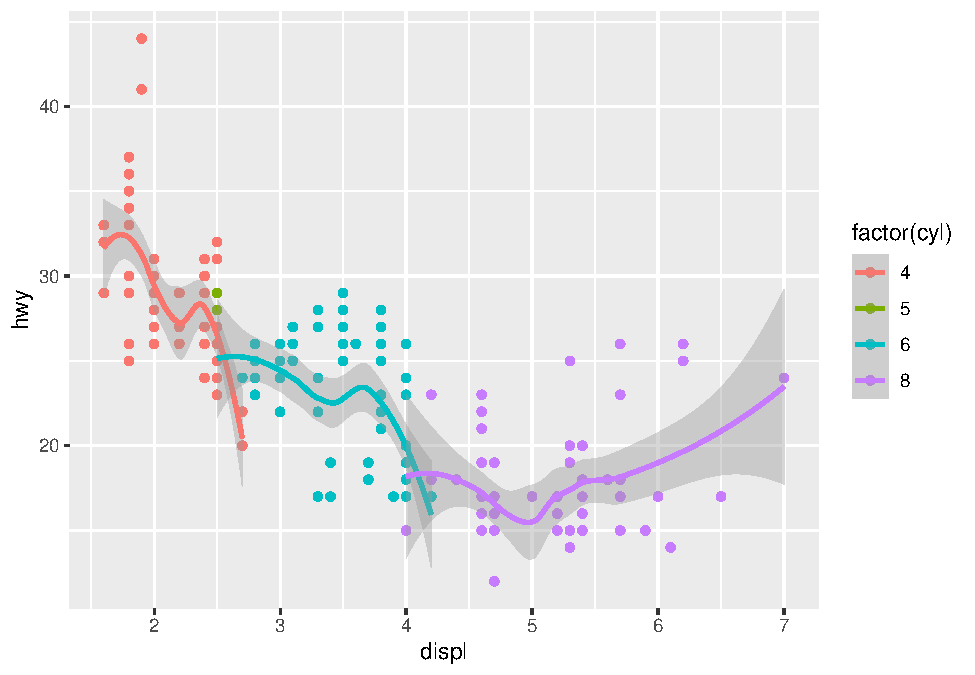
\includegraphics{_main_files/figure-latex/unnamed-chunk-3-1.pdf}

如果需要对整体数据进行平滑,可将colour参数设置在散点图层内而非第一层,这样第三层的平滑图形就不会受到colour参数的影响。

\begin{Shaded}
\begin{Highlighting}[]
\NormalTok{p }\OtherTok{\textless{}{-}} \FunctionTok{ggplot}\NormalTok{(mpg,}\FunctionTok{aes}\NormalTok{(}\AttributeTok{x=}\NormalTok{displ,}\AttributeTok{y=}\NormalTok{hwy))}
\NormalTok{p }\SpecialCharTok{+} \FunctionTok{geom\_point}\NormalTok{(}\FunctionTok{aes}\NormalTok{(}\AttributeTok{colour=}\FunctionTok{factor}\NormalTok{(cyl))) }\SpecialCharTok{+} \FunctionTok{geom\_smooth}\NormalTok{()}
\end{Highlighting}
\end{Shaded}

\begin{verbatim}
## `geom_smooth()` using method = 'loess' and formula 'y ~ x'
\end{verbatim}

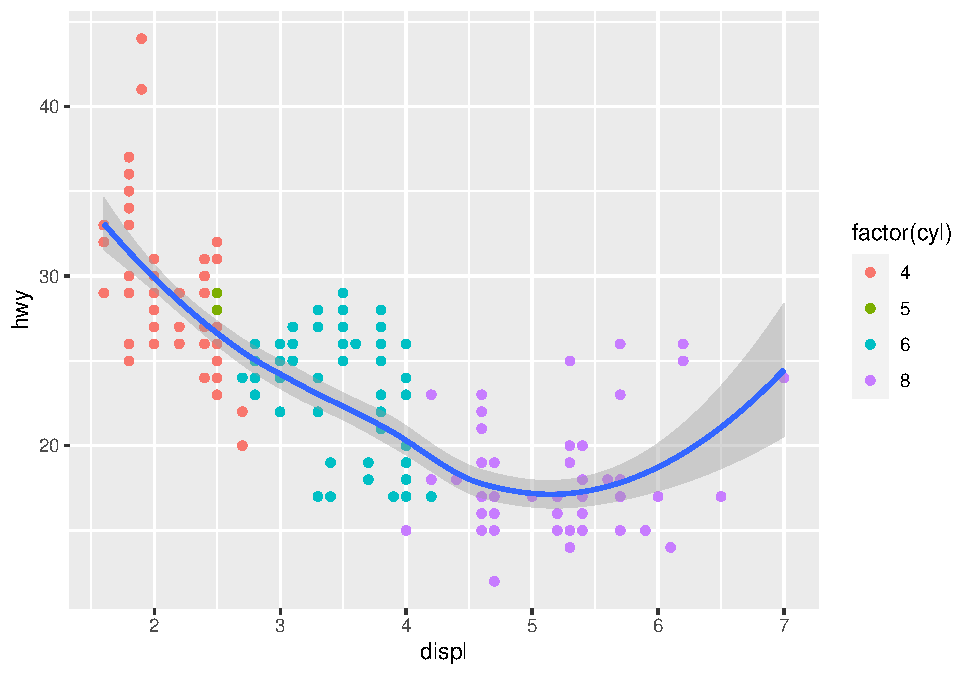
\includegraphics{_main_files/figure-latex/unnamed-chunk-4-1.pdf}

\hypertarget{ux76f8ux5173ux56feux5f62}{%
\subsection{相关图形}\label{ux76f8ux5173ux56feux5f62}}

\hypertarget{ux56feux5c42ux63a7ux5236ux4e0eux76f4ux65b9ux56fe}{%
\subsubsection{图层控制与直方图}\label{ux56feux5c42ux63a7ux5236ux4e0eux76f4ux65b9ux56fe}}

第一层必须是原始数据层,其中data参数控制数据来源,注意数据形式只能是数据框格式。aes参数控制了对哪些变量进行图形映射,以及映射方式,aes是Aesthetic的缩写。\\
下面我们来绘制一个直方图作为示例。数据集仍采取mpg,对hwy变量绘制直方图。首先加载了扩展包,然后用ggplot函数建立了第一层,hwy数据映射到X轴上;使用+号增加了第二层,即直方图对象层。此时p被视为一种层对象,使用summary函数可得到关于它的更多信息,print(p)命令即可进行绘图。

\begin{Shaded}
\begin{Highlighting}[]
\FunctionTok{library}\NormalTok{(ggplot2)}
\NormalTok{p }\OtherTok{\textless{}{-}} \FunctionTok{ggplot}\NormalTok{(}\AttributeTok{data =}\NormalTok{ mpg,}\FunctionTok{aes}\NormalTok{(}\AttributeTok{x =}\NormalTok{ hwy))}
\NormalTok{p }\OtherTok{\textless{}{-}}\NormalTok{ p }\SpecialCharTok{+} \FunctionTok{geom\_histogram}\NormalTok{()}
\FunctionTok{summary}\NormalTok{(p)}
\end{Highlighting}
\end{Shaded}

\begin{verbatim}
## data: manufacturer, model, displ, year, cyl, trans, drv, cty, hwy, fl,
##   class [234x11]
## mapping:  x = ~hwy
## faceting: <ggproto object: Class FacetNull, Facet, gg>
##     compute_layout: function
##     draw_back: function
##     draw_front: function
##     draw_labels: function
##     draw_panels: function
##     finish_data: function
##     init_scales: function
##     map_data: function
##     params: list
##     setup_data: function
##     setup_params: function
##     shrink: TRUE
##     train_scales: function
##     vars: function
##     super:  <ggproto object: Class FacetNull, Facet, gg>
## -----------------------------------
## geom_bar: na.rm = FALSE, orientation = NA
## stat_bin: binwidth = NULL, bins = NULL, na.rm = FALSE, orientation = NA, pad = FALSE
## position_stack
\end{verbatim}

\begin{Shaded}
\begin{Highlighting}[]
\FunctionTok{print}\NormalTok{(p)}
\end{Highlighting}
\end{Shaded}

\begin{verbatim}
## `stat_bin()` using `bins = 30`. Pick better value with `binwidth`.
\end{verbatim}

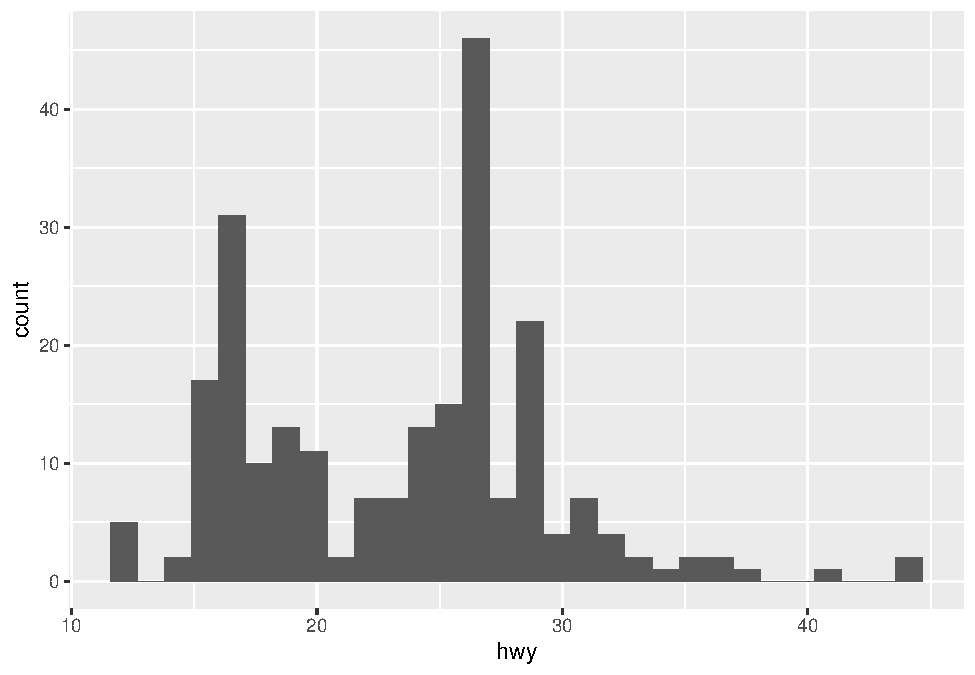
\includegraphics{_main_files/figure-latex/unnamed-chunk-5-1.pdf}

p对象含有两层,第一层数据层描述了变量和映射方式,第二层是直方图对象(geom\_histogram),geom表示几何对象,它是ggplot中重要的图层控制对象,因为它负责图形渲染的类型。geom\_histogram是图形渲染类型的一种。

每个geom对象都需要有数据输入,数据可以从第一层中自动读取,也可以在aes参数中直接设置。而且每个geom还默认搭配某种统计变换(stat),geom\_histogram的默认统计变换是stat\_bin。它负责对数据进行分组计数。

下面我们尝试两种更为复杂的直方图,首先将数据按照year这个变量划分为两组,用不同的颜色绘制直方图,而且用频率而非计数来刻画Y轴,并添加密度曲线。

\begin{Shaded}
\begin{Highlighting}[]
\NormalTok{p }\OtherTok{\textless{}{-}} \FunctionTok{ggplot}\NormalTok{(mpg,}\FunctionTok{aes}\NormalTok{(hwy))}
\NormalTok{p }\SpecialCharTok{+} \FunctionTok{geom\_histogram}\NormalTok{(}\AttributeTok{position =} \StringTok{\textquotesingle{}identity\textquotesingle{}}\NormalTok{,}
\AttributeTok{alpha=}\FloatTok{0.5}\NormalTok{,}
\FunctionTok{aes}\NormalTok{(}\AttributeTok{y =}\NormalTok{ ..density..,}
\AttributeTok{fill =} \FunctionTok{factor}\NormalTok{(year))) }\SpecialCharTok{+}
\FunctionTok{stat\_density}\NormalTok{(}\AttributeTok{geom =} \StringTok{\textquotesingle{}line\textquotesingle{}}\NormalTok{,}
\AttributeTok{position =} \StringTok{\textquotesingle{}identity\textquotesingle{}}\NormalTok{,}
\FunctionTok{aes}\NormalTok{(}\AttributeTok{colour =} \FunctionTok{factor}\NormalTok{(year)))}
\end{Highlighting}
\end{Shaded}

\begin{verbatim}
## `stat_bin()` using `bins = 30`. Pick better value with `binwidth`.
\end{verbatim}

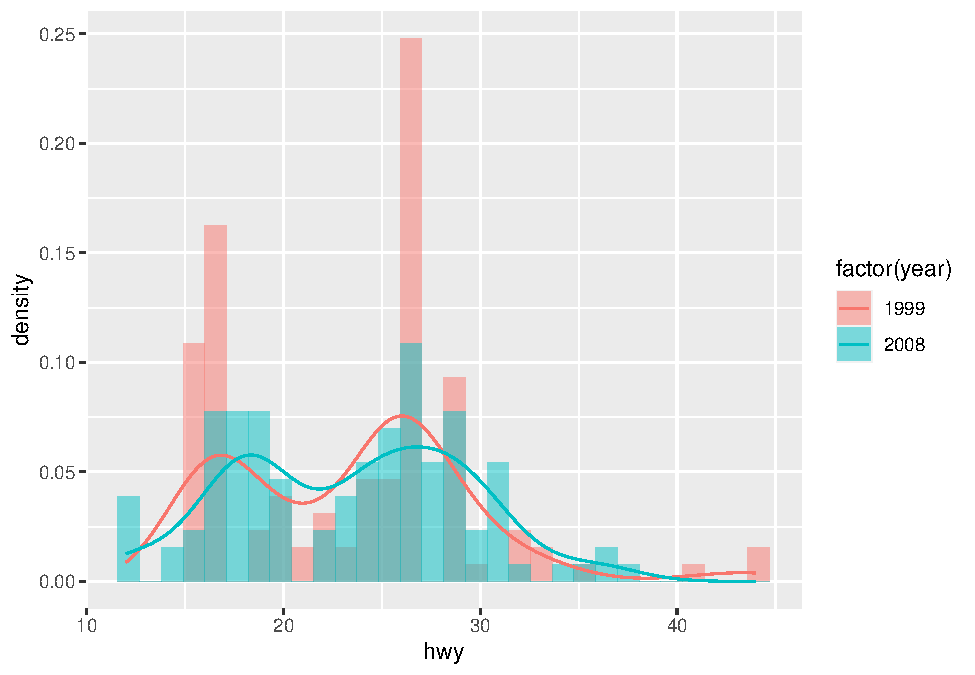
\includegraphics{_main_files/figure-latex/unnamed-chunk-6-1.pdf}

\hypertarget{ux4f4dux7f6eux8c03ux6574ux4e0eux6761ux5f62ux56fe}{%
\subsubsection{位置调整与条形图}\label{ux4f4dux7f6eux8c03ux6574ux4e0eux6761ux5f62ux56fe}}

位置调整(Position adjustments)是针对同一图层内元素的位置进行微调的方法。它包括五种设置,分别是stack、dodge、fill、identity、jitter。

我们用条形图来展示其用法,仍使用mpg数据集,其中用到的变量是class,即生产汽车的类型,以及year生产年份。下面的条形图是将各类型的汽车数量进行汇集,并以年份作为分组变量。我们首先载入扩展包,然后用频数表对数据进行大致的了解,最后绘制了四种条形图。

\begin{Shaded}
\begin{Highlighting}[]
\FunctionTok{library}\NormalTok{(ggplot2)}
\FunctionTok{with}\NormalTok{(mpg,}\FunctionTok{table}\NormalTok{(class,year))}
\end{Highlighting}
\end{Shaded}

\begin{verbatim}
##             year
## class        1999 2008
##   2seater       2    3
##   compact      25   22
##   midsize      20   21
##   minivan       6    5
##   pickup       16   17
##   subcompact   19   16
##   suv          29   33
\end{verbatim}

\begin{Shaded}
\begin{Highlighting}[]
\NormalTok{p }\OtherTok{\textless{}{-}} \FunctionTok{ggplot}\NormalTok{(}\AttributeTok{data=}\NormalTok{mpg,}\FunctionTok{aes}\NormalTok{(}\AttributeTok{x=}\NormalTok{class,}\AttributeTok{fill=}\FunctionTok{factor}\NormalTok{(year)))}
\NormalTok{p }\SpecialCharTok{+} \FunctionTok{geom\_bar}\NormalTok{(}\AttributeTok{position=}\StringTok{\textquotesingle{}dodge\textquotesingle{}}\NormalTok{)}
\end{Highlighting}
\end{Shaded}

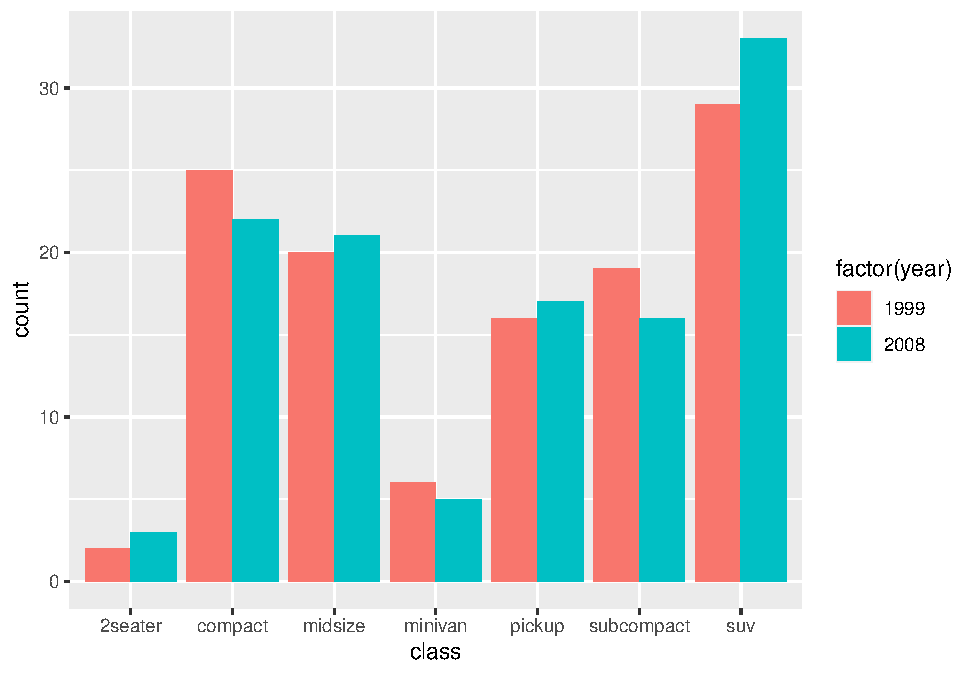
\includegraphics{_main_files/figure-latex/unnamed-chunk-7-1.pdf}

\begin{Shaded}
\begin{Highlighting}[]
\NormalTok{p }\SpecialCharTok{+} \FunctionTok{geom\_bar}\NormalTok{(}\AttributeTok{position=}\StringTok{\textquotesingle{}stack\textquotesingle{}}\NormalTok{)}
\end{Highlighting}
\end{Shaded}

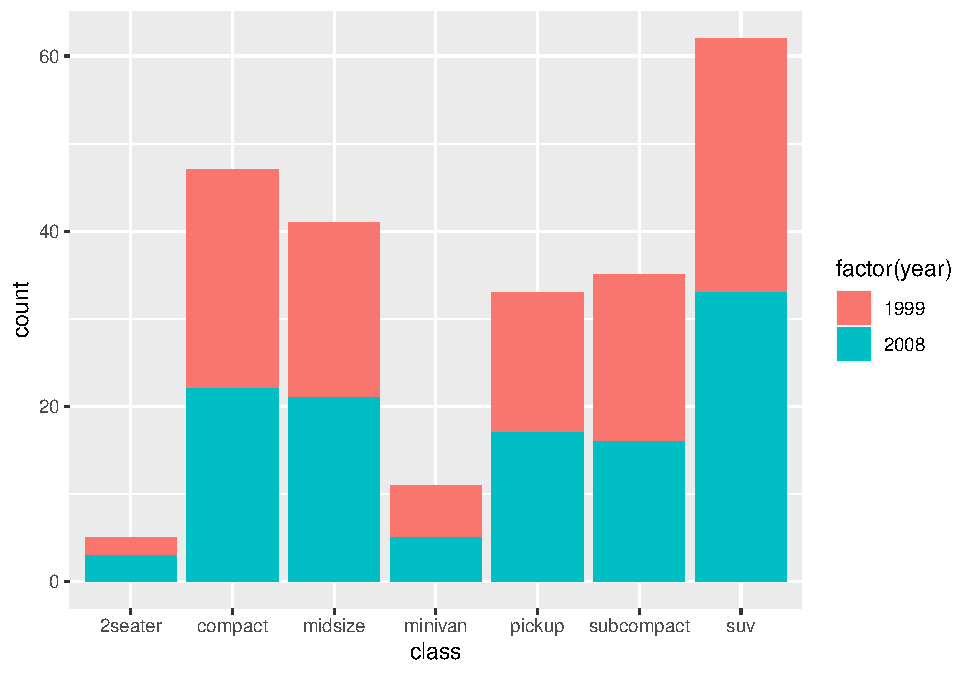
\includegraphics{_main_files/figure-latex/unnamed-chunk-7-2.pdf}

\begin{Shaded}
\begin{Highlighting}[]
\NormalTok{p }\SpecialCharTok{+} \FunctionTok{geom\_bar}\NormalTok{(}\AttributeTok{position=}\StringTok{\textquotesingle{}fill\textquotesingle{}}\NormalTok{)}
\end{Highlighting}
\end{Shaded}

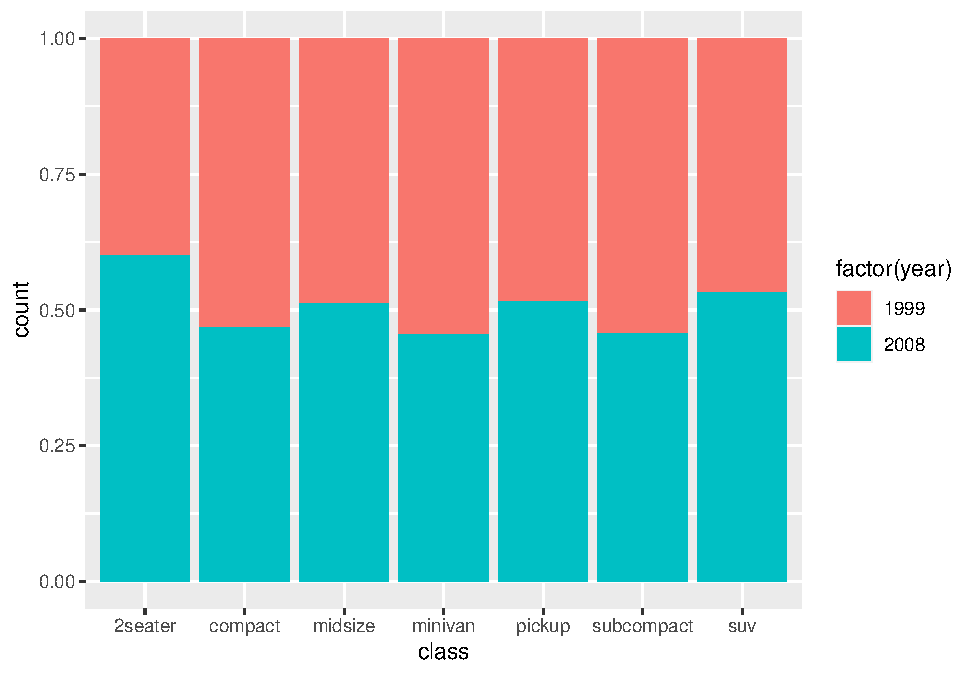
\includegraphics{_main_files/figure-latex/unnamed-chunk-7-3.pdf}

\begin{Shaded}
\begin{Highlighting}[]
\NormalTok{p }\SpecialCharTok{+} \FunctionTok{geom\_bar}\NormalTok{(}\AttributeTok{position=}\StringTok{\textquotesingle{}identity\textquotesingle{}}\NormalTok{,}\AttributeTok{alpha=}\FloatTok{0.3}\NormalTok{)}
\end{Highlighting}
\end{Shaded}

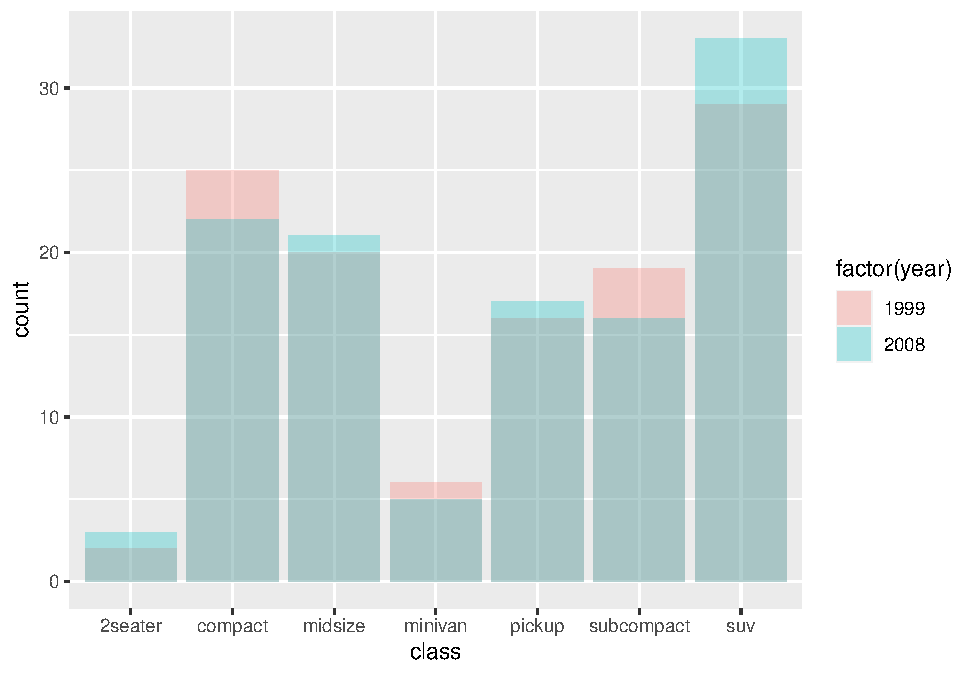
\includegraphics{_main_files/figure-latex/unnamed-chunk-7-4.pdf}

可以看到dodge方式是将不同年份的数据并列放置;stack方式是将不同年份数据推叠放置,这也是geom\_bar的默认处理方式;fill方式和stack类似,但Y轴不再是计数,而是以百分比显示;identity方式是不做任何改变直接显示出来,所以需要设置透明度才能看得清楚。

\hypertarget{ux6563ux70b9ux56fe}{%
\subsubsection{散点图}\label{ux6563ux70b9ux56fe}}

\begin{itemize}
\tightlist
\item
  色彩和形状的控制
\end{itemize}

数据特征不仅可以用坐标来表示,也可以用不同的色彩或形状来表示。仍以mpg数据集为例,所用到的变量有cty(城市中行驶距离),hwy(高速路行驶距离),displ(排量大小),year(生产年份)

\begin{Shaded}
\begin{Highlighting}[]
\FunctionTok{library}\NormalTok{(ggplot2)}
\NormalTok{p }\OtherTok{\textless{}{-}} \FunctionTok{ggplot}\NormalTok{(mpg, }\FunctionTok{aes}\NormalTok{(cty, hwy))}
\NormalTok{p1 }\OtherTok{\textless{}{-}}\NormalTok{ p }\SpecialCharTok{+} \FunctionTok{geom\_point}\NormalTok{(}\FunctionTok{aes}\NormalTok{(}\AttributeTok{colour =} \FunctionTok{factor}\NormalTok{(year),}\AttributeTok{shape =} \FunctionTok{factor}\NormalTok{(year), }\AttributeTok{size =}\NormalTok{ displ), }\AttributeTok{alpha =} \FloatTok{0.6}\NormalTok{, }\AttributeTok{position =} \StringTok{\textquotesingle{}jitter\textquotesingle{}}\NormalTok{)}
\FunctionTok{print}\NormalTok{(p1)}
\end{Highlighting}
\end{Shaded}

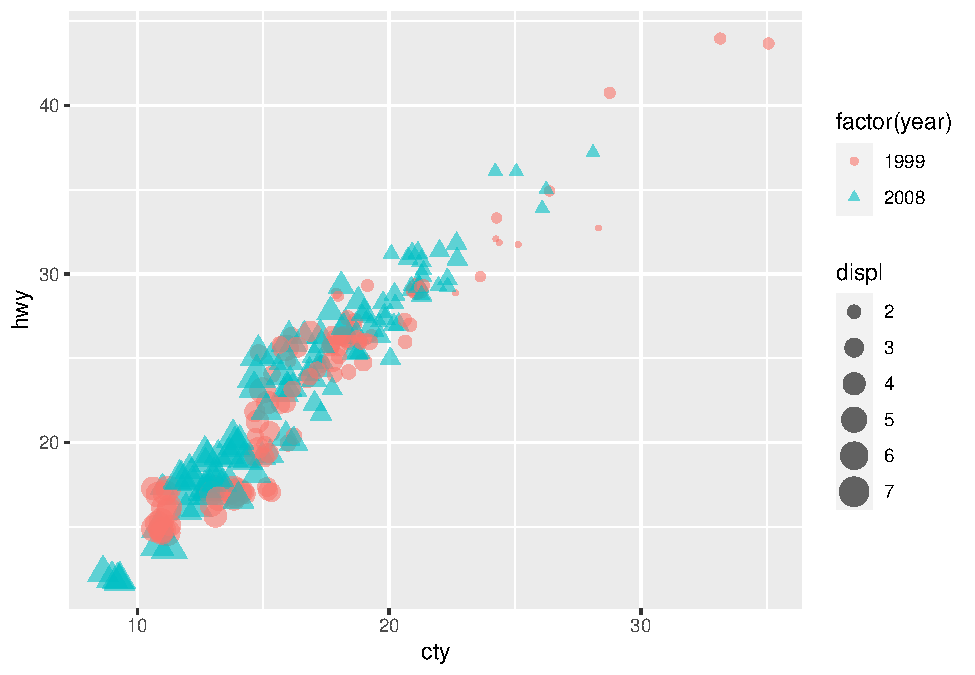
\includegraphics{_main_files/figure-latex/unnamed-chunk-8-1.pdf}

我们将1999年生产车型用红色圆形表示,2008年用兰色三角形表示,排量用图形的大小表示,并且设置了透明度和jitter以避免样本点之间的重叠。可观察到2008年生产的大排量车型较多,从而油耗较高,单位油耗行驶距离较短。

\begin{itemize}
\tightlist
\item
  坐标的控制
\end{itemize}

上图右上角数据点较为稀疏,这种情况下可用对数变换。为了演示ggplot2对图形坐标的控制,我们对X轴和Y轴均进行对数变换,然后对X轴的坐标显示加以限制,只显示X轴数据的均值,以及一倍标准差的坐标。

\begin{Shaded}
\begin{Highlighting}[]
\NormalTok{cty.mean}\OtherTok{=}\FunctionTok{with}\NormalTok{(mpg,}\FunctionTok{mean}\NormalTok{(cty))}
\NormalTok{cty.sd}\OtherTok{=}\FunctionTok{with}\NormalTok{(mpg,}\FunctionTok{sd}\NormalTok{(cty))}
\NormalTok{p1 }\SpecialCharTok{+} \FunctionTok{scale\_x\_continuous}\NormalTok{(}\AttributeTok{trans=}\StringTok{\textquotesingle{}log\textquotesingle{}}\NormalTok{,}\AttributeTok{breaks=}\FunctionTok{c}\NormalTok{(cty.mean}\SpecialCharTok{{-}}\NormalTok{cty.sd,cty.mean,cty.mean}\SpecialCharTok{+}\NormalTok{cty.sd), }\AttributeTok{labels=}\FunctionTok{c}\NormalTok{(}\StringTok{"high"}\NormalTok{, }\StringTok{"mean"}\NormalTok{, }\StringTok{"low"}\NormalTok{)) }\SpecialCharTok{+} \FunctionTok{scale\_y\_continuous}\NormalTok{(}\AttributeTok{trans=}\StringTok{\textquotesingle{}log\textquotesingle{}}\NormalTok{)}
\end{Highlighting}
\end{Shaded}

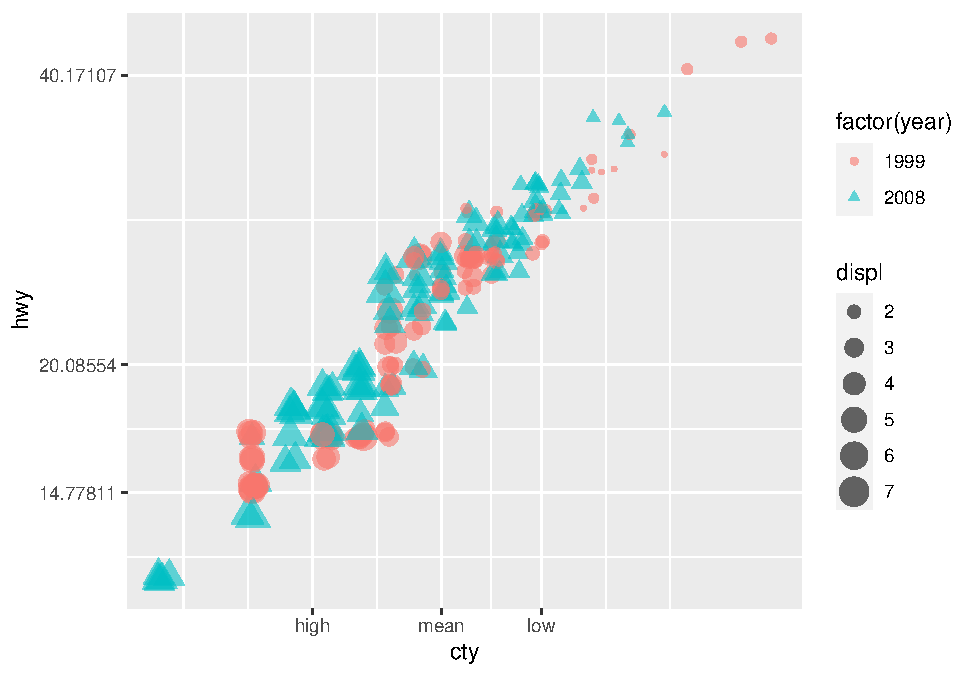
\includegraphics{_main_files/figure-latex/unnamed-chunk-9-1.pdf}

\begin{itemize}
\tightlist
\item
  文字说明
\end{itemize}

利用geom\_text函数可添加文字说明以增强图形的可读性

\begin{Shaded}
\begin{Highlighting}[]
\NormalTok{p }\OtherTok{\textless{}{-}} \FunctionTok{ggplot}\NormalTok{(mtcars, }\FunctionTok{aes}\NormalTok{(}\AttributeTok{x=}\NormalTok{wt, }\AttributeTok{y=}\NormalTok{mpg,}\AttributeTok{colour=}\FunctionTok{factor}\NormalTok{(cyl),}\AttributeTok{label=}\FunctionTok{rownames}\NormalTok{(mtcars)))}
\NormalTok{p }\SpecialCharTok{+} \FunctionTok{geom\_text}\NormalTok{(}\AttributeTok{hjust=}\DecValTok{0}\NormalTok{,}\AttributeTok{vjust=}\SpecialCharTok{{-}}\DecValTok{1}\NormalTok{,}\AttributeTok{alpha=}\FloatTok{0.8}\NormalTok{)}\SpecialCharTok{+} \FunctionTok{geom\_point}\NormalTok{(}\AttributeTok{size=}\DecValTok{3}\NormalTok{,}\FunctionTok{aes}\NormalTok{(}\AttributeTok{shape=}\FunctionTok{factor}\NormalTok{(cyl)))}
\end{Highlighting}
\end{Shaded}

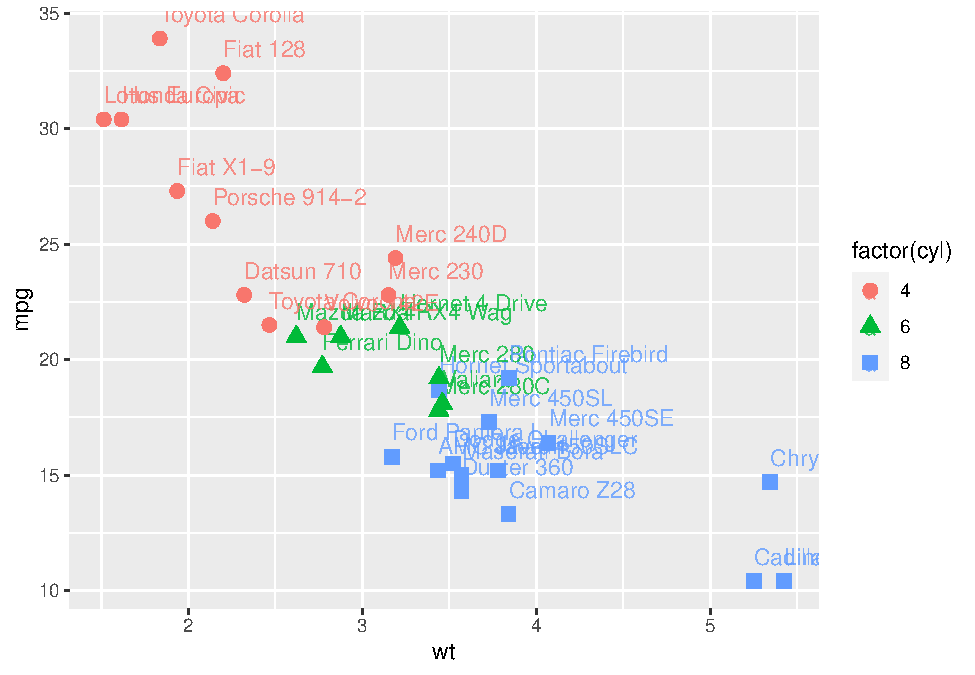
\includegraphics{_main_files/figure-latex/unnamed-chunk-10-1.pdf}

\hypertarget{ggplot2ux7ed8ux5236ux65f6ux95f4ux5e8fux5217ux53d8ux5316ux56fe}{%
\subsection{ggplot2绘制时间序列变化图}\label{ggplot2ux7ed8ux5236ux65f6ux95f4ux5e8fux5217ux53d8ux5316ux56fe}}

ggplot2包也能对时间序列数据绘图,但在处理上需要有些注意的地方,可能需要注意转化成data.frame。ggplot()可以先将时间序列类型拆成数据框类型然后再绘图。

\href{https://www.sodic.com.cn/datasets}{数据来源:2021全球开放数据应用创新大赛https://www.sodic.com.cn/datasets}

\hypertarget{shiny-appux6574ux4f53ux4ecbux7ecd}{%
\chapter{Shiny APP整体介绍}\label{shiny-appux6574ux4f53ux4ecbux7ecd}}

\textbf{详细内容请参考学习网址\href{https://mastering-shiny.org}{Mastering Shiny} }

\hypertarget{ux57faux672cux4ecbux7ecd}{%
\section{基本介绍}\label{ux57faux672cux4ecbux7ecd}}

创建Shiny APP有多种方法,最简单的方法是为你的文件创建一个新的目录,并放入一个app.R的文件,app.R的文件整体布局如下:

\texttt{library(shiny)}(加载Shiny包)

\texttt{ui\ \textless{}-\ fluidPage()}(定义用户界面)

\texttt{server\ \textless{}-\ function(input,\ output,\ session)\ \{\}}(定义服务器功能)

\texttt{shinyApp(ui,\ server)}(从ui和server构建并启动一个shiny应用程序)

\hypertarget{ux6dfbux52a0ux7528ux6237ux754cux9762ux63a7ux4ef6}{%
\subsection{添加用户界面控件}\label{ux6dfbux52a0ux7528ux6237ux754cux9762ux63a7ux4ef6}}

例如:

\begin{Shaded}
\begin{Highlighting}[]
\FunctionTok{library}\NormalTok{(shiny)}
\NormalTok{ui }\OtherTok{\textless{}{-}} \FunctionTok{fluidPage}\NormalTok{(}
  \FunctionTok{selectInput}\NormalTok{(}\StringTok{"dataset"}\NormalTok{, }\AttributeTok{label =} \StringTok{"Dataset"}\NormalTok{, }\AttributeTok{choices =} \FunctionTok{ls}\NormalTok{(}\StringTok{"package:datasets"}\NormalTok{)),}
  \FunctionTok{verbatimTextOutput}\NormalTok{(}\StringTok{"summary"}\NormalTok{),}
  \FunctionTok{tableOutput}\NormalTok{(}\StringTok{"table"}\NormalTok{)}
\NormalTok{)}
\end{Highlighting}
\end{Shaded}

这里fluidPage()是一个布局函数,用于设置页面的基本视觉结构。

selectInput()是一个输入控件,允许用户通过提供一个值与应用程序进行交互。

verbatimTextOutput()和tableOutput()是输出控件,它们告诉Shiny将渲染输出放在哪里。

verbatimTextOutput()显示代码,tableOutput()显示表格。

\hypertarget{ux5728ux670dux52a1ux5668ux51fdux6570ux4e2dux5b9aux4e49ux8f93ux51faux6dfbux52a0ux884cux4e3a}{%
\subsection{在服务器函数中定义输出(添加行为)}\label{ux5728ux670dux52a1ux5668ux51fdux6570ux4e2dux5b9aux4e49ux8f93ux51faux6dfbux52a0ux884cux4e3a}}

Shiny使用反应式编程使应用程序具有交互性。

例如:

\begin{Shaded}
\begin{Highlighting}[]
\NormalTok{server }\OtherTok{\textless{}{-}} \ControlFlowTok{function}\NormalTok{(input, output, session) \{}
\NormalTok{  output}\SpecialCharTok{$}\NormalTok{summary }\OtherTok{\textless{}{-}} \FunctionTok{renderPrint}\NormalTok{(\{}
\NormalTok{    dataset }\OtherTok{\textless{}{-}} \FunctionTok{get}\NormalTok{(input}\SpecialCharTok{$}\NormalTok{dataset, }\StringTok{"package:datasets"}\NormalTok{)}
    \FunctionTok{summary}\NormalTok{(dataset)}
\NormalTok{  \})}
  
\NormalTok{  output}\SpecialCharTok{$}\NormalTok{table }\OtherTok{\textless{}{-}} \FunctionTok{renderTable}\NormalTok{(\{}
\NormalTok{    dataset }\OtherTok{\textless{}{-}} \FunctionTok{get}\NormalTok{(input}\SpecialCharTok{$}\NormalTok{dataset, }\StringTok{"package:datasets"}\NormalTok{)}
\NormalTok{    dataset}
\NormalTok{  \})}
\NormalTok{\}}
\end{Highlighting}
\end{Shaded}

使用特定的render函数来包装您提供的一些代码。

renderPrint()与verbatimTextOutput()配对以显示具有固定宽度(逐字)文本的统计摘要,renderTable()与tableOutput()配对以显示表格中的输入数据。

\hypertarget{ux521bux5efashinyux5e94ux7528ux7a0bux5e8f}{%
\subsection{创建Shiny应用程序}\label{ux521bux5efashinyux5e94ux7528ux7a0bux5e8f}}

\begin{Shaded}
\begin{Highlighting}[]
\FunctionTok{shinyApp}\NormalTok{(}\AttributeTok{ui=}\NormalTok{ui, }\AttributeTok{server=}\NormalTok{server)}
\end{Highlighting}
\end{Shaded}

\begin{verbatim}
## PhantomJS not found. You can install it with webshot::install_phantomjs(). If it is installed, please make sure the phantomjs executable can be found via the PATH variable.
\end{verbatim}

\hypertarget{ux524dux7aefux4ecbux7ecdux7528ux6237ux7aefui}{%
\section{前端介绍(用户端UI)}\label{ux524dux7aefux4ecbux7ecdux7528ux6237ux7aefui}}

\hypertarget{inputs}{%
\subsection{inputs}\label{inputs}}

\emph{sliderInput}

\emph{textInput}

\emph{passwordInput}

\emph{textAreaInput}

\emph{numericInput}

\emph{dateInput}

\emph{dateRangeInput}

\emph{selectInput}

\emph{radioButtons}

\emph{checkboxGroupInput}

\emph{checkboxInput}

\emph{fileInput}

\emph{actionButton}

具体应用\textbf{代码}请参考{[}\url{https://shiny.rstudio.com/gallery/widget-gallery.html}{]}\url{https://shiny.rstudio.com/gallery/widget-gallery.html}

\hypertarget{outputs}{%
\subsection{outputs}\label{outputs}}

\hypertarget{text}{%
\subsubsection{Text}\label{text}}

\emph{textOutput()}

\emph{verbatimTextOutput()}

renderText()将结果组合成一个字符串,通常与textOutput()配对;renderPrint()打印结果,通常与verbatimTextOutput()配对。

\begin{Shaded}
\begin{Highlighting}[]
\NormalTok{ui }\OtherTok{\textless{}{-}} \FunctionTok{fluidPage}\NormalTok{(}
  \FunctionTok{textOutput}\NormalTok{(}\StringTok{"text"}\NormalTok{),}
  \FunctionTok{verbatimTextOutput}\NormalTok{(}\StringTok{"code"}\NormalTok{)}
\NormalTok{)}
\NormalTok{server }\OtherTok{\textless{}{-}} \ControlFlowTok{function}\NormalTok{(input, output, session) \{}
\NormalTok{  output}\SpecialCharTok{$}\NormalTok{text }\OtherTok{\textless{}{-}} \FunctionTok{renderText}\NormalTok{(\{ }
    \StringTok{"Hello friend!"} 
\NormalTok{  \})}
\NormalTok{  output}\SpecialCharTok{$}\NormalTok{code }\OtherTok{\textless{}{-}} \FunctionTok{renderPrint}\NormalTok{(\{ }
    \FunctionTok{summary}\NormalTok{(}\DecValTok{1}\SpecialCharTok{:}\DecValTok{10}\NormalTok{) }
\NormalTok{  \})}
\NormalTok{\}}
\end{Highlighting}
\end{Shaded}

\hypertarget{tables}{%
\subsubsection{Tables}\label{tables}}

\emph{tableOutput()}

\emph{dataTableOutput()}

tableOutput()和renderTable()呈现一个静态数据表,一次显示所有数据;dataTableOutput()和renderDataTable()呈现一个动态表,显示固定数量的行以及用于更改哪些行可见的控件。

\begin{Shaded}
\begin{Highlighting}[]
\NormalTok{ui }\OtherTok{\textless{}{-}} \FunctionTok{fluidPage}\NormalTok{(}
  \FunctionTok{tableOutput}\NormalTok{(}\StringTok{"static"}\NormalTok{),}
  \FunctionTok{dataTableOutput}\NormalTok{(}\StringTok{"dynamic"}\NormalTok{)}
\NormalTok{)}
\NormalTok{server }\OtherTok{\textless{}{-}} \ControlFlowTok{function}\NormalTok{(input, output, session) \{}
\NormalTok{  output}\SpecialCharTok{$}\NormalTok{static }\OtherTok{\textless{}{-}} \FunctionTok{renderTable}\NormalTok{(}\FunctionTok{head}\NormalTok{(mtcars))}
\NormalTok{  output}\SpecialCharTok{$}\NormalTok{dynamic }\OtherTok{\textless{}{-}} \FunctionTok{renderDataTable}\NormalTok{(mtcars, }\AttributeTok{options =} \FunctionTok{list}\NormalTok{(}\AttributeTok{pageLength =} \DecValTok{5}\NormalTok{))}
\NormalTok{\}}
\end{Highlighting}
\end{Shaded}

\hypertarget{plots}{%
\subsubsection{Plots}\label{plots}}

\emph{plotOutput()}

plotOutput() 常与renderPlot()对应;

\begin{Shaded}
\begin{Highlighting}[]
\NormalTok{ui }\OtherTok{\textless{}{-}} \FunctionTok{fluidPage}\NormalTok{(}
  \FunctionTok{plotOutput}\NormalTok{(}\StringTok{"plot"}\NormalTok{, }\AttributeTok{width =} \StringTok{"400px"}\NormalTok{)}
\NormalTok{)}
\NormalTok{server }\OtherTok{\textless{}{-}} \ControlFlowTok{function}\NormalTok{(input, output, session) \{}
\NormalTok{  output}\SpecialCharTok{$}\NormalTok{plot }\OtherTok{\textless{}{-}} \FunctionTok{renderPlot}\NormalTok{(}\FunctionTok{plot}\NormalTok{(}\DecValTok{1}\SpecialCharTok{:}\DecValTok{5}\NormalTok{), }\AttributeTok{res =} \DecValTok{96}\NormalTok{)}
\NormalTok{\}}
\end{Highlighting}
\end{Shaded}

\hypertarget{downloads}{%
\subsubsection{Downloads}\label{downloads}}

\emph{downloadButton()}

\emph{downloadLink()}

\hypertarget{ux53cdux5e94ux5f0fux7f16ux7a0b}{%
\section{反应式编程}\label{ux53cdux5e94ux5f0fux7f16ux7a0b}}

\hypertarget{inputs-1}{%
\subsection{inputs}\label{inputs-1}}

注意事项:

1.与典型的列表不同,输入对象是只读的,不可以修改服务器函数内部的输入。

2.它对允许谁阅读它是有选择性的。要读取输入,必须处于由render\ldots()或reactive()等函数创建的反应上下文中。

\hypertarget{output}{%
\subsection{output}\label{output}}

输出与输入非常相似:它也是一个类似列表的对象,根据输出ID命名。主要区别在于,使用它来发送输出,而不是接收输入。

\hypertarget{reactive-programming}{%
\subsection{Reactive programming}\label{reactive-programming}}

既有input又有output的应用程序

\textbf{注意:}

如果运行一个Shiny应用程序,代码永远不会运行,仔细检查ui用户界面和server服务器功能使用相同的标识符。

reactive()可以简化许多重复步骤。

\begin{Shaded}
\begin{Highlighting}[]
\NormalTok{server }\OtherTok{\textless{}{-}} \ControlFlowTok{function}\NormalTok{(input, output, session) \{}
\NormalTok{  x1 }\OtherTok{\textless{}{-}} \FunctionTok{reactive}\NormalTok{(}\FunctionTok{rnorm}\NormalTok{(input}\SpecialCharTok{$}\NormalTok{n1, input}\SpecialCharTok{$}\NormalTok{mean1, input}\SpecialCharTok{$}\NormalTok{sd1))}
\NormalTok{  x2 }\OtherTok{\textless{}{-}} \FunctionTok{reactive}\NormalTok{(}\FunctionTok{rnorm}\NormalTok{(input}\SpecialCharTok{$}\NormalTok{n2, input}\SpecialCharTok{$}\NormalTok{mean2, input}\SpecialCharTok{$}\NormalTok{sd2))}

\NormalTok{  output}\SpecialCharTok{$}\NormalTok{hist }\OtherTok{\textless{}{-}} \FunctionTok{renderPlot}\NormalTok{(\{}
    \FunctionTok{freqpoly}\NormalTok{(}\FunctionTok{x1}\NormalTok{(), }\FunctionTok{x2}\NormalTok{(), }\AttributeTok{binwidth =}\NormalTok{ input}\SpecialCharTok{$}\NormalTok{binwidth, }\AttributeTok{xlim =}\NormalTok{ input}\SpecialCharTok{$}\NormalTok{range)}
\NormalTok{  \}, }\AttributeTok{res =} \DecValTok{96}\NormalTok{)}

\NormalTok{  output}\SpecialCharTok{$}\NormalTok{ttest }\OtherTok{\textless{}{-}} \FunctionTok{renderText}\NormalTok{(\{}
    \FunctionTok{t\_test}\NormalTok{(}\FunctionTok{x1}\NormalTok{(), }\FunctionTok{x2}\NormalTok{())}
\NormalTok{  \})}
\NormalTok{\}}
\end{Highlighting}
\end{Shaded}

假设您想通过不断地重新模拟数据来强化这是模拟数据的事实,以便您看到的是动画而不是静态绘图,可以用一个新的函数来增加更新的频率:reactiveTimer()。

\begin{Shaded}
\begin{Highlighting}[]
\NormalTok{server }\OtherTok{\textless{}{-}} \ControlFlowTok{function}\NormalTok{(input, output, session) \{}
\NormalTok{  timer }\OtherTok{\textless{}{-}} \FunctionTok{reactiveTimer}\NormalTok{(}\DecValTok{500}\NormalTok{)}
  
\NormalTok{  x1 }\OtherTok{\textless{}{-}} \FunctionTok{reactive}\NormalTok{(\{}
    \FunctionTok{timer}\NormalTok{()}
    \FunctionTok{rpois}\NormalTok{(input}\SpecialCharTok{$}\NormalTok{n, input}\SpecialCharTok{$}\NormalTok{lambda1)}
\NormalTok{  \})}
\NormalTok{  x2 }\OtherTok{\textless{}{-}} \FunctionTok{reactive}\NormalTok{(\{}
    \FunctionTok{timer}\NormalTok{()}
    \FunctionTok{rpois}\NormalTok{(input}\SpecialCharTok{$}\NormalTok{n, input}\SpecialCharTok{$}\NormalTok{lambda2)}
\NormalTok{  \})}
  
\NormalTok{  output}\SpecialCharTok{$}\NormalTok{hist }\OtherTok{\textless{}{-}} \FunctionTok{renderPlot}\NormalTok{(\{}
    \FunctionTok{freqpoly}\NormalTok{(}\FunctionTok{x1}\NormalTok{(), }\FunctionTok{x2}\NormalTok{(), }\AttributeTok{binwidth =} \DecValTok{1}\NormalTok{, }\AttributeTok{xlim =} \FunctionTok{c}\NormalTok{(}\DecValTok{0}\NormalTok{, }\DecValTok{40}\NormalTok{))}
\NormalTok{  \}, }\AttributeTok{res =} \DecValTok{96}\NormalTok{)}
\NormalTok{\}}
\end{Highlighting}
\end{Shaded}

若选择执行昂贵的计算,可以使用是actionButton():

\begin{Shaded}
\begin{Highlighting}[]
\NormalTok{ui }\OtherTok{\textless{}{-}} \FunctionTok{fluidPage}\NormalTok{(}
  \FunctionTok{fluidRow}\NormalTok{(}
    \FunctionTok{column}\NormalTok{(}\DecValTok{3}\NormalTok{, }
      \FunctionTok{numericInput}\NormalTok{(}\StringTok{"lambda1"}\NormalTok{, }\AttributeTok{label =} \StringTok{"lambda1"}\NormalTok{, }\AttributeTok{value =} \DecValTok{3}\NormalTok{),}
      \FunctionTok{numericInput}\NormalTok{(}\StringTok{"lambda2"}\NormalTok{, }\AttributeTok{label =} \StringTok{"lambda2"}\NormalTok{, }\AttributeTok{value =} \DecValTok{5}\NormalTok{),}
      \FunctionTok{numericInput}\NormalTok{(}\StringTok{"n"}\NormalTok{, }\AttributeTok{label =} \StringTok{"n"}\NormalTok{, }\AttributeTok{value =} \FloatTok{1e4}\NormalTok{, }\AttributeTok{min =} \DecValTok{0}\NormalTok{),}
      \FunctionTok{actionButton}\NormalTok{(}\StringTok{"simulate"}\NormalTok{, }\StringTok{"Simulate!"}\NormalTok{)}
\NormalTok{    ),}
    \FunctionTok{column}\NormalTok{(}\DecValTok{9}\NormalTok{, }\FunctionTok{plotOutput}\NormalTok{(}\StringTok{"hist"}\NormalTok{))}
\NormalTok{  )}
\NormalTok{)}
\NormalTok{server }\OtherTok{\textless{}{-}} \ControlFlowTok{function}\NormalTok{(input, output, session) \{}
\NormalTok{  x1 }\OtherTok{\textless{}{-}} \FunctionTok{eventReactive}\NormalTok{(input}\SpecialCharTok{$}\NormalTok{simulate, \{}
    \FunctionTok{rpois}\NormalTok{(input}\SpecialCharTok{$}\NormalTok{n, input}\SpecialCharTok{$}\NormalTok{lambda1)}
\NormalTok{  \})}
\NormalTok{  x2 }\OtherTok{\textless{}{-}} \FunctionTok{eventReactive}\NormalTok{(input}\SpecialCharTok{$}\NormalTok{simulate, \{}
    \FunctionTok{rpois}\NormalTok{(input}\SpecialCharTok{$}\NormalTok{n, input}\SpecialCharTok{$}\NormalTok{lambda2)}
\NormalTok{  \})}

\NormalTok{  output}\SpecialCharTok{$}\NormalTok{hist }\OtherTok{\textless{}{-}} \FunctionTok{renderPlot}\NormalTok{(\{}
    \FunctionTok{freqpoly}\NormalTok{(}\FunctionTok{x1}\NormalTok{(), }\FunctionTok{x2}\NormalTok{(), }\AttributeTok{binwidth =} \DecValTok{1}\NormalTok{, }\AttributeTok{xlim =} \FunctionTok{c}\NormalTok{(}\DecValTok{0}\NormalTok{, }\DecValTok{40}\NormalTok{))}
\NormalTok{  \}, }\AttributeTok{res =} \DecValTok{96}\NormalTok{)}
\NormalTok{\}}
\end{Highlighting}
\end{Shaded}

需要eventReactive(),它有两个参数:第一个参数指定依赖什么,第二个参数指定计算什么。这使得该应用程序在单击模拟时只能计算x1()和x2()。

\hypertarget{shiny-feedback}{%
\chapter{Shiny feedback}\label{shiny-feedback}}

\hypertarget{validation}{%
\section{Validation}\label{validation}}

\hypertarget{validating-input}{%
\subsection{Validating input}\label{validating-input}}

无效的输入可能会导致不想向用户显示的非信息性错误。为了阻止输入触发反应性变化您需要一个新工具:req()

\begin{Shaded}
\begin{Highlighting}[]
\FunctionTok{library}\NormalTok{(shiny)}

\NormalTok{ui }\OtherTok{\textless{}{-}} \FunctionTok{fluidPage}\NormalTok{(}
\NormalTok{  shinyFeedback}\SpecialCharTok{::}\FunctionTok{useShinyFeedback}\NormalTok{(),}
  \FunctionTok{numericInput}\NormalTok{(}\StringTok{"n"}\NormalTok{,}\StringTok{"n"}\NormalTok{,}\AttributeTok{value=}\DecValTok{10}\NormalTok{),}
  \FunctionTok{textOutput}\NormalTok{(}\StringTok{"half"}\NormalTok{)}
  
\NormalTok{)}

\NormalTok{server }\OtherTok{\textless{}{-}} \ControlFlowTok{function}\NormalTok{(input, output, session) \{}
\NormalTok{  half}\OtherTok{\textless{}{-}}\FunctionTok{reactive}\NormalTok{(\{}
\NormalTok{    even}\OtherTok{\textless{}{-}}\NormalTok{input}\SpecialCharTok{$}\NormalTok{n }\SpecialCharTok{\%\%} \DecValTok{2}\SpecialCharTok{==}\DecValTok{0}
\NormalTok{    shinyFeedback}\SpecialCharTok{::}\FunctionTok{feedbackWarning}\NormalTok{(}\StringTok{"n"}\NormalTok{,}\SpecialCharTok{!}\NormalTok{even,}\StringTok{"please select an even number!"}\NormalTok{)}
    \CommentTok{\#req(even)}
\NormalTok{    input}\SpecialCharTok{$}\NormalTok{n }\SpecialCharTok{/}\DecValTok{2}
    
\NormalTok{  \})}
\NormalTok{    output}\SpecialCharTok{$}\NormalTok{half}\OtherTok{\textless{}{-}}\FunctionTok{renderText}\NormalTok{(}\FunctionTok{half}\NormalTok{())}
  
\NormalTok{\}}
\end{Highlighting}
\end{Shaded}

\hypertarget{cancelling-execution-with-req}{%
\subsection{Cancelling execution with req()}\label{cancelling-execution-with-req}}

\begin{Shaded}
\begin{Highlighting}[]
\FunctionTok{library}\NormalTok{(shiny)}

\NormalTok{ui }\OtherTok{\textless{}{-}} \FunctionTok{fluidPage}\NormalTok{(}
  \FunctionTok{selectInput}\NormalTok{(}\StringTok{"language"}\NormalTok{,}\StringTok{"Language"}\NormalTok{,}\AttributeTok{choices =} \FunctionTok{c}\NormalTok{(}\StringTok{""}\NormalTok{,}\StringTok{"English"}\NormalTok{,}\StringTok{"Maori"}\NormalTok{)),}
  \FunctionTok{textInput}\NormalTok{(}\StringTok{"name"}\NormalTok{,}\StringTok{"Name"}\NormalTok{),}
  \FunctionTok{textOutput}\NormalTok{(}\StringTok{"greeting"}\NormalTok{)}
  
\NormalTok{)}

\NormalTok{server }\OtherTok{\textless{}{-}} \ControlFlowTok{function}\NormalTok{(input, output, session) \{}
\NormalTok{  greetings}\OtherTok{\textless{}{-}}\FunctionTok{c}\NormalTok{(}
    \AttributeTok{Engilsh=}\StringTok{"Hello"}\NormalTok{,}
    \AttributeTok{Maori=}\StringTok{"Kia ora"}
\NormalTok{  )}
\NormalTok{  output}\SpecialCharTok{$}\NormalTok{greeting}\OtherTok{\textless{}{-}}\FunctionTok{renderText}\NormalTok{(\{}
    \CommentTok{\#req(input$language,input$name)}
    \FunctionTok{paste0}\NormalTok{(greetings[[input}\SpecialCharTok{$}\NormalTok{language]],}\StringTok{""}\NormalTok{,input}\SpecialCharTok{$}\NormalTok{name,}\StringTok{"!"}\NormalTok{)}
\NormalTok{  \})}
\NormalTok{\}}
\end{Highlighting}
\end{Shaded}

\hypertarget{req-and-validation}{%
\subsection{req() and validation}\label{req-and-validation}}

结合req()和shinyFeedback来解决一个更具挑战性的问题

注意cancelOutput = TRUE的用法:通常取消无功会复位所有下游输出;使用cancelOutput = TRUE会让它们显示最后一个good value

\begin{Shaded}
\begin{Highlighting}[]
\FunctionTok{library}\NormalTok{(shiny)}

\NormalTok{ui }\OtherTok{\textless{}{-}} \FunctionTok{fluidPage}\NormalTok{(}
\NormalTok{  shinyFeedback}\SpecialCharTok{::}\FunctionTok{useShinyFeedback}\NormalTok{(),}
   \FunctionTok{textInput}\NormalTok{(}\StringTok{"dataset"}\NormalTok{, }\StringTok{"Dataset name"}\NormalTok{), }
  \FunctionTok{tableOutput}\NormalTok{(}\StringTok{"data"}\NormalTok{)}
\NormalTok{)}

\NormalTok{server }\OtherTok{\textless{}{-}} \ControlFlowTok{function}\NormalTok{(input, output, session) \{}
\NormalTok{  data}\OtherTok{\textless{}{-}}\FunctionTok{reactive}\NormalTok{(\{}
    \FunctionTok{req}\NormalTok{(input}\SpecialCharTok{$}\NormalTok{dataset)}
    
\NormalTok{    exists}\OtherTok{\textless{}{-}}\FunctionTok{exists}\NormalTok{(input}\SpecialCharTok{$}\NormalTok{dataset,}\StringTok{"package:datasets"}\NormalTok{)}
\NormalTok{    shinyFeedback}\SpecialCharTok{::}\FunctionTok{feedbackDanger}\NormalTok{(}\StringTok{"dataset"}\NormalTok{,}\SpecialCharTok{!}\NormalTok{exists,}\StringTok{"Unknown dataset"}\NormalTok{)}
    \FunctionTok{req}\NormalTok{(exists,}\AttributeTok{cancelOutput =} \ConstantTok{TRUE}\NormalTok{)}
    
    \FunctionTok{get}\NormalTok{(input}\SpecialCharTok{$}\NormalTok{dataset, }\StringTok{"package:datasets"}\NormalTok{)}
    
\NormalTok{  \})}
  
\NormalTok{  output}\SpecialCharTok{$}\NormalTok{data}\OtherTok{\textless{}{-}}\FunctionTok{renderTable}\NormalTok{(\{}
    \FunctionTok{head}\NormalTok{(}\FunctionTok{data}\NormalTok{())}
\NormalTok{  \})}
\NormalTok{\}}
\end{Highlighting}
\end{Shaded}

\hypertarget{validate-output}{%
\subsection{Validate output}\label{validate-output}}

使用内置于shiny: validate()中的工具
validate(message)停止执行代码的其余部分

\begin{Shaded}
\begin{Highlighting}[]
\FunctionTok{library}\NormalTok{(shiny)}

\NormalTok{ui }\OtherTok{\textless{}{-}} \FunctionTok{fluidPage}\NormalTok{(}
  \FunctionTok{numericInput}\NormalTok{(}\StringTok{"x"}\NormalTok{,}\StringTok{"x"}\NormalTok{,}\AttributeTok{value=}\DecValTok{0}\NormalTok{),}
  \FunctionTok{selectInput}\NormalTok{(}\StringTok{"trans"}\NormalTok{,}\StringTok{"transformation"}\NormalTok{,}\AttributeTok{choices=}\FunctionTok{c}\NormalTok{(}\StringTok{"square"}\NormalTok{, }\StringTok{"log"}\NormalTok{, }\StringTok{"square{-}root"}\NormalTok{)),}
  \FunctionTok{textOutput}\NormalTok{(}\StringTok{"out"}\NormalTok{)}
\NormalTok{)}

\NormalTok{server }\OtherTok{\textless{}{-}} \ControlFlowTok{function}\NormalTok{(input, output, session) \{}
  
\NormalTok{ output}\SpecialCharTok{$}\NormalTok{out }\OtherTok{\textless{}{-}} \FunctionTok{renderText}\NormalTok{(\{}
    \ControlFlowTok{if}\NormalTok{ (input}\SpecialCharTok{$}\NormalTok{x }\SpecialCharTok{\textless{}} \DecValTok{0} \SpecialCharTok{\&\&}\NormalTok{ input}\SpecialCharTok{$}\NormalTok{trans }\SpecialCharTok{\%in\%} \FunctionTok{c}\NormalTok{(}\StringTok{"log"}\NormalTok{, }\StringTok{"square{-}root"}\NormalTok{)) \{}
      \FunctionTok{validate}\NormalTok{(}\StringTok{"x can not be negative for this transformation"}\NormalTok{)}
\NormalTok{    \}}
   
   \ControlFlowTok{switch}\NormalTok{(input}\SpecialCharTok{$}\NormalTok{trans,}
      \AttributeTok{square =}\NormalTok{ input}\SpecialCharTok{$}\NormalTok{x }\SpecialCharTok{\^{}} \DecValTok{2}\NormalTok{,}
      \StringTok{"square{-}root"} \OtherTok{=} \FunctionTok{sqrt}\NormalTok{(input}\SpecialCharTok{$}\NormalTok{x),}
      \AttributeTok{log =} \FunctionTok{log}\NormalTok{(input}\SpecialCharTok{$}\NormalTok{x)}
\NormalTok{    )}
\NormalTok{  \})}
\NormalTok{\}}
\end{Highlighting}
\end{Shaded}

\hypertarget{notifications}{%
\section{Notifications}\label{notifications}}

\hypertarget{transient-notification}{%
\subsection{Transient notification}\label{transient-notification}}

\hypertarget{removing-on-completion}{%
\subsection{Removing on completion}\label{removing-on-completion}}

将持续时间设置为空(duration = NULL),将关闭按钮设置为假closeButton = FALSE,以便在任务完成之前通知保持可见。
在任务开始时显示通知,并在任务完成时删除通知\\
使用on.exit(),它确保无论任务如何完成(成功完成或出现错误),通知都会被删除\\
on.exit:ensures that the notification is removed

\hypertarget{shiny-uploads-and-downloads}{%
\chapter{Shiny uploads and downloads}\label{shiny-uploads-and-downloads}}

\hypertarget{upload}{%
\section{upload}\label{upload}}

\begin{Shaded}
\begin{Highlighting}[]
\FunctionTok{library}\NormalTok{(shiny)}

\NormalTok{ui }\OtherTok{\textless{}{-}} \FunctionTok{fluidPage}\NormalTok{(}
  \FunctionTok{fileInput}\NormalTok{(}\StringTok{"upload"}\NormalTok{,}\ConstantTok{NULL}\NormalTok{,}\AttributeTok{buttonLabel=}\StringTok{"Upload..."}\NormalTok{, }\AttributeTok{multiple =} \ConstantTok{TRUE}\NormalTok{),}
  \FunctionTok{tableOutput}\NormalTok{(}\StringTok{"files"}\NormalTok{)}
\NormalTok{)}

\NormalTok{server }\OtherTok{\textless{}{-}} \ControlFlowTok{function}\NormalTok{(input, output, session) \{}
\NormalTok{  output}\SpecialCharTok{$}\NormalTok{files}\OtherTok{\textless{}{-}}\FunctionTok{renderTable}\NormalTok{(input}\SpecialCharTok{$}\NormalTok{upload)}
\NormalTok{\}}
\end{Highlighting}
\end{Shaded}

在页面加载时,input\(upload被初始化为空,所以需要req(input\)upload)来确保您代码等待直到第一个文件被上传

accept参数允许您限制可能的输入。最简单的方法是提供文件扩展名的字符向量,如accept = ``.csv''。但是accept参数只是给浏览器的一个建议,并不总是被强制执行。

在R中获取文件扩展名最简单的方法是tools::file\_ext()

\begin{Shaded}
\begin{Highlighting}[]
\FunctionTok{library}\NormalTok{(shiny)}

\NormalTok{ui }\OtherTok{\textless{}{-}} \FunctionTok{fluidPage}\NormalTok{(}
  \FunctionTok{fileInput}\NormalTok{(}\StringTok{"upload"}\NormalTok{,}\ConstantTok{NULL}\NormalTok{,}\AttributeTok{accept =} \FunctionTok{c}\NormalTok{(}\StringTok{".csv"}\NormalTok{,}\StringTok{".tsv"}\NormalTok{)),}
  \FunctionTok{numericInput}\NormalTok{(}\StringTok{"n"}\NormalTok{,}\StringTok{"Rows"}\NormalTok{,}\AttributeTok{value=}\DecValTok{5}\NormalTok{, }\AttributeTok{min =} \DecValTok{1}\NormalTok{, }\AttributeTok{step =} \DecValTok{1}\NormalTok{),}
  \FunctionTok{tableOutput}\NormalTok{(}\StringTok{"head"}\NormalTok{)}
\NormalTok{)}

\NormalTok{server }\OtherTok{\textless{}{-}} \ControlFlowTok{function}\NormalTok{(input, output, session) \{}
\NormalTok{  data}\OtherTok{\textless{}{-}}\FunctionTok{reactive}\NormalTok{(\{}
    \FunctionTok{req}\NormalTok{(input}\SpecialCharTok{$}\NormalTok{pload)}
    
\NormalTok{    ext}\OtherTok{\textless{}{-}}\NormalTok{tools}\SpecialCharTok{::}\FunctionTok{file\_ext}\NormalTok{()}
    \ControlFlowTok{switch}\NormalTok{(ext,}
           \AttributeTok{csv=}\NormalTok{vroom}\SpecialCharTok{::}\FunctionTok{vroom}\NormalTok{(input}\SpecialCharTok{$}\NormalTok{upload}\SpecialCharTok{$}\NormalTok{datapath,}\AttributeTok{delim=}\StringTok{","}\NormalTok{),}
             \AttributeTok{tsv=}\NormalTok{vroom}\SpecialCharTok{::}\FunctionTok{vroom}\NormalTok{(input}\SpecialCharTok{$}\NormalTok{upload}\SpecialCharTok{$}\NormalTok{datapath,}\AttributeTok{delim=}\StringTok{"}\SpecialCharTok{\textbackslash{}t}\StringTok{"}\NormalTok{),}
             \FunctionTok{validate}\NormalTok{(}\StringTok{"Invalid file; Please upload a .csv or .tsv file"}\NormalTok{))}
\NormalTok{  \})}
\NormalTok{  output}\SpecialCharTok{$}\NormalTok{head}\OtherTok{\textless{}{-}}\FunctionTok{renderTable}\NormalTok{(\{}
    \FunctionTok{head}\NormalTok{(}\FunctionTok{data}\NormalTok{(),input}\SpecialCharTok{$}\NormalTok{n)}
\NormalTok{  \})}
\NormalTok{\}}
\end{Highlighting}
\end{Shaded}

\hypertarget{download}{%
\section{Download}\label{download}}

用户界面很简单:使用downloadButton(id)或downloadLink(id)给用户一些东西来点击下载文件

与其他输出不同,downloadButton()没有与渲染函数配对,可以使用downloadHandler()

downloadHandler()有两个参数,都是函数:filename是一个没有参数的函数,它返回一个文件名(作为字符串),此功能的工作是创建将在下载对话框中显示给用户的名称。content应该是带有一个参数file的函数,file是保存文件的路径。这个函数的工作是将文件保存在Shiny知道的地方,这样它就可以将文件发送给用户

\begin{Shaded}
\begin{Highlighting}[]
\FunctionTok{library}\NormalTok{(shiny)}

\NormalTok{ui }\OtherTok{\textless{}{-}} \FunctionTok{fluidPage}\NormalTok{(}
  \FunctionTok{selectInput}\NormalTok{(}\StringTok{"dataset"}\NormalTok{, }\StringTok{"Pick a dataset"}\NormalTok{, }\FunctionTok{ls}\NormalTok{(}\StringTok{"package:datasets"}\NormalTok{)),}
  \FunctionTok{tableOutput}\NormalTok{(}\StringTok{"preview"}\NormalTok{),}
  \FunctionTok{downloadButton}\NormalTok{(}\StringTok{"download"}\NormalTok{,}\StringTok{"Download.tsv"}\NormalTok{)}
\NormalTok{)}

\NormalTok{server }\OtherTok{\textless{}{-}} \ControlFlowTok{function}\NormalTok{(input, output, session) \{}
\NormalTok{   data }\OtherTok{\textless{}{-}} \FunctionTok{reactive}\NormalTok{(\{}
\NormalTok{    out }\OtherTok{\textless{}{-}} \FunctionTok{get}\NormalTok{(input}\SpecialCharTok{$}\NormalTok{dataset, }\StringTok{"package:datasets"}\NormalTok{)}
    \ControlFlowTok{if}\NormalTok{ (}\SpecialCharTok{!}\FunctionTok{is.data.frame}\NormalTok{(out)) \{}
      \FunctionTok{validate}\NormalTok{(}\FunctionTok{paste0}\NormalTok{(}\StringTok{"\textquotesingle{}"}\NormalTok{, input}\SpecialCharTok{$}\NormalTok{dataset, }\StringTok{"\textquotesingle{} is not a data frame"}\NormalTok{))}
\NormalTok{    \}}
\NormalTok{    out}
\NormalTok{  \})}
  
\NormalTok{  output}\SpecialCharTok{$}\NormalTok{preview }\OtherTok{\textless{}{-}} \FunctionTok{renderTable}\NormalTok{(\{}
    \FunctionTok{head}\NormalTok{(}\FunctionTok{data}\NormalTok{())}
\NormalTok{  \})}
    
\NormalTok{  output}\SpecialCharTok{$}\NormalTok{download }\OtherTok{\textless{}{-}} \FunctionTok{downloadHandler}\NormalTok{(}
    \AttributeTok{filename =} \ControlFlowTok{function}\NormalTok{() \{}
      \FunctionTok{paste0}\NormalTok{(input}\SpecialCharTok{$}\NormalTok{dataset, }\StringTok{".tsv"}\NormalTok{)}
\NormalTok{    \},}
    \AttributeTok{content =} \ControlFlowTok{function}\NormalTok{(file) \{}
\NormalTok{      vroom}\SpecialCharTok{::}\FunctionTok{vroom\_write}\NormalTok{(}\FunctionTok{data}\NormalTok{(), file)}
\NormalTok{    \}}
\NormalTok{  )}
\NormalTok{\}}
\end{Highlighting}
\end{Shaded}

\hypertarget{downloading-reports}{%
\section{Downloading reports}\label{downloading-reports}}

生成报告的一个强大方法是使用参数化的RMarkdown文档。参数化的RMarkdown文件在YAML元数据中有一个参数字段

\begin{Shaded}
\begin{Highlighting}[]
\FunctionTok{library}\NormalTok{(shiny)}

\NormalTok{ui }\OtherTok{\textless{}{-}} \FunctionTok{fluidPage}\NormalTok{(}
  \FunctionTok{sliderInput}\NormalTok{(}\StringTok{"n"}\NormalTok{, }\StringTok{"Number of points"}\NormalTok{, }\DecValTok{1}\NormalTok{, }\DecValTok{100}\NormalTok{, }\DecValTok{50}\NormalTok{),}
  \FunctionTok{downloadButton}\NormalTok{(}\StringTok{"report"}\NormalTok{, }\StringTok{"Generate report"}\NormalTok{)}
\NormalTok{)}

\NormalTok{server }\OtherTok{\textless{}{-}} \ControlFlowTok{function}\NormalTok{(input, output, session) \{}
\NormalTok{  output}\SpecialCharTok{$}\NormalTok{report }\OtherTok{\textless{}{-}} \FunctionTok{downloadHandler}\NormalTok{(}
    \AttributeTok{filename =} \StringTok{"report.html"}\NormalTok{,}
    \AttributeTok{content =} \ControlFlowTok{function}\NormalTok{(file) \{}
\NormalTok{      params }\OtherTok{\textless{}{-}} \FunctionTok{list}\NormalTok{(}\AttributeTok{n =}\NormalTok{ input}\SpecialCharTok{$}\NormalTok{n)}
      
\NormalTok{      id }\OtherTok{\textless{}{-}} \FunctionTok{showNotification}\NormalTok{(}
        \StringTok{"Rendering report..."}\NormalTok{, }
        \AttributeTok{duration =} \ConstantTok{NULL}\NormalTok{, }
        \AttributeTok{closeButton =} \ConstantTok{FALSE}
\NormalTok{      )}
      \FunctionTok{on.exit}\NormalTok{(}\FunctionTok{removeNotification}\NormalTok{(id), }\AttributeTok{add =} \ConstantTok{TRUE}\NormalTok{)}

\NormalTok{      rmarkdown}\SpecialCharTok{::}\FunctionTok{render}\NormalTok{(}\StringTok{"report.Rmd"}\NormalTok{, }
        \AttributeTok{output\_file =}\NormalTok{ file,}
        \AttributeTok{params =}\NormalTok{ params,}
        \AttributeTok{envir =} \FunctionTok{new.env}\NormalTok{(}\AttributeTok{parent =} \FunctionTok{globalenv}\NormalTok{())}
\NormalTok{      )}
\NormalTok{    \}}
\NormalTok{  )}
\NormalTok{\}}
\end{Highlighting}
\end{Shaded}

\hypertarget{dynamic-ui}{%
\chapter{Dynamic UI}\label{dynamic-ui}}

创建动态用户界面有三种关键技术:

\emph{使用update更新函数族修改输入控件的参数}

\emph{使用tabsetPanel()有条件地显示和隐藏部分用户界面}

\emph{使用uiOutput()和renderUI()用代码生成用户界面的选定部分}

\hypertarget{updating-inputs}{%
\section{Updating inputs}\label{updating-inputs}}

\begin{Shaded}
\begin{Highlighting}[]
\FunctionTok{library}\NormalTok{(shiny)}

\NormalTok{ui }\OtherTok{\textless{}{-}} \FunctionTok{fluidPage}\NormalTok{(}
  \FunctionTok{numericInput}\NormalTok{(}\StringTok{"n"}\NormalTok{,}\StringTok{"Simulations"}\NormalTok{,}\DecValTok{10}\NormalTok{),}
  \FunctionTok{actionButton}\NormalTok{(}\StringTok{"simulate"}\NormalTok{,}\StringTok{"Simulate"}\NormalTok{)}
\NormalTok{)}

\NormalTok{server }\OtherTok{\textless{}{-}} \ControlFlowTok{function}\NormalTok{(input, output, session) \{}
  \FunctionTok{observeEvent}\NormalTok{(input}\SpecialCharTok{$}\NormalTok{n, \{}
\NormalTok{    label}\OtherTok{\textless{}{-}}\FunctionTok{paste0}\NormalTok{(}\StringTok{"Simulate"}\NormalTok{,input}\SpecialCharTok{$}\NormalTok{n,}\StringTok{"times"}\NormalTok{)}
    \FunctionTok{updateActionButton}\NormalTok{(}\AttributeTok{inputId =} \StringTok{"simulate"}\NormalTok{,}\AttributeTok{label=}\NormalTok{label)}
\NormalTok{  \})}
\NormalTok{\}}
\end{Highlighting}
\end{Shaded}

\begin{Shaded}
\begin{Highlighting}[]
\FunctionTok{library}\NormalTok{(shiny)}

\NormalTok{ui }\OtherTok{\textless{}{-}} \FunctionTok{fluidPage}\NormalTok{(}
  \FunctionTok{selectInput}\NormalTok{(}\StringTok{"dataset"}\NormalTok{,}\StringTok{"Choose a dataset"}\NormalTok{,}\FunctionTok{c}\NormalTok{(}\StringTok{"pressure"}\NormalTok{,}\StringTok{"cars"}\NormalTok{)),}
  \FunctionTok{selectInput}\NormalTok{(}\StringTok{"column"}\NormalTok{,}\StringTok{"Choose column"}\NormalTok{,}\FunctionTok{character}\NormalTok{(}\DecValTok{0}\NormalTok{)),}
  \FunctionTok{verbatimTextOutput}\NormalTok{(}\StringTok{"summary"}\NormalTok{)}
\NormalTok{)}

\NormalTok{server }\OtherTok{\textless{}{-}} \ControlFlowTok{function}\NormalTok{(input, output, session) \{}
  \CommentTok{\# freezeReactiveValue(input,"column")}
\NormalTok{  dataset}\OtherTok{\textless{}{-}}\FunctionTok{reactive}\NormalTok{(}\FunctionTok{get}\NormalTok{(input}\SpecialCharTok{$}\NormalTok{dataset,}\StringTok{"package:datasets"}\NormalTok{))}
  
  \FunctionTok{observeEvent}\NormalTok{(input}\SpecialCharTok{$}\NormalTok{dataset,\{}
    \FunctionTok{updateSelectInput}\NormalTok{(}\AttributeTok{inputId =} \StringTok{"column"}\NormalTok{,}\AttributeTok{choices =} \FunctionTok{names}\NormalTok{(}\FunctionTok{dataset}\NormalTok{()))}
\NormalTok{  \})}
\NormalTok{  output}\SpecialCharTok{$}\NormalTok{summary}\OtherTok{\textless{}{-}}\FunctionTok{renderPrint}\NormalTok{(\{}
    \FunctionTok{summary}\NormalTok{(}\FunctionTok{dataset}\NormalTok{()[[input}\SpecialCharTok{$}\NormalTok{column]])}
\NormalTok{  \})}
\NormalTok{\}}
\end{Highlighting}
\end{Shaded}

\hypertarget{dynamic-visibility}{%
\section{Dynamic visibility}\label{dynamic-visibility}}

\begin{Shaded}
\begin{Highlighting}[]
\FunctionTok{library}\NormalTok{(shiny)}

\NormalTok{ui }\OtherTok{\textless{}{-}} \FunctionTok{fluidPage}\NormalTok{(}
  \FunctionTok{sidebarLayout}\NormalTok{(}
    \FunctionTok{sidebarPanel}\NormalTok{(}
      \FunctionTok{selectInput}\NormalTok{(}\StringTok{"controller"}\NormalTok{,}\StringTok{"Show"}\NormalTok{,}\AttributeTok{choices =} \FunctionTok{paste0}\NormalTok{(}\StringTok{"panel"}\NormalTok{,}\DecValTok{1}\SpecialCharTok{:}\DecValTok{3}\NormalTok{))}
\NormalTok{    ),}
    \FunctionTok{mainPanel}\NormalTok{(}
      \FunctionTok{tabsetPanel}\NormalTok{(}
        \AttributeTok{id=}\StringTok{"switcher"}\NormalTok{,}
        \AttributeTok{type=}\StringTok{"hidden"}\NormalTok{,}
        \FunctionTok{tabPanelBody}\NormalTok{(}\StringTok{"panel1"}\NormalTok{,}\StringTok{"Panel 1 content"}\NormalTok{),}
        \FunctionTok{tabPanelBody}\NormalTok{(}\StringTok{"panel2"}\NormalTok{,}\StringTok{"Panel 2 content"}\NormalTok{),}
        \FunctionTok{tabPanelBody}\NormalTok{(}\StringTok{"panel3"}\NormalTok{,}\StringTok{"Panel 3 content"}\NormalTok{)}
\NormalTok{      )}
\NormalTok{    )}
\NormalTok{  )}
\NormalTok{)}

\NormalTok{server }\OtherTok{\textless{}{-}} \ControlFlowTok{function}\NormalTok{(input, output, session) \{}
  \FunctionTok{observeEvent}\NormalTok{(input}\SpecialCharTok{$}\NormalTok{controller,\{}
    \FunctionTok{updateTabsetPanel}\NormalTok{(}\AttributeTok{inputId =} \StringTok{"switcher"}\NormalTok{,}\AttributeTok{selected=}\NormalTok{input}\SpecialCharTok{$}\NormalTok{controller)}
\NormalTok{  \})}
\NormalTok{\}}
\end{Highlighting}
\end{Shaded}

\begin{Shaded}
\begin{Highlighting}[]
\FunctionTok{library}\NormalTok{(shiny)}

\NormalTok{ui }\OtherTok{\textless{}{-}} \FunctionTok{fluidPage}\NormalTok{(}
  \FunctionTok{sidebarLayout}\NormalTok{(}
    \FunctionTok{sidebarPanel}\NormalTok{(}
      \FunctionTok{selectInput}\NormalTok{(}\StringTok{"dist"}\NormalTok{,}\StringTok{"Distribution"}\NormalTok{,}
                  \AttributeTok{choices=}\FunctionTok{c}\NormalTok{(}\StringTok{"normal"}\NormalTok{,}\StringTok{"uniform"}\NormalTok{,}\StringTok{"exponential"}\NormalTok{)),}
      \FunctionTok{numericInput}\NormalTok{(}\StringTok{"n"}\NormalTok{,}\StringTok{"Number of samples"}\NormalTok{,}\AttributeTok{value=}\DecValTok{100}\NormalTok{),}
\NormalTok{      parameter\_tabs}\OtherTok{\textless{}{-}}\FunctionTok{tabsetPanel}\NormalTok{(}
        \AttributeTok{id=}\StringTok{"params"}\NormalTok{,}
        \AttributeTok{type=}\StringTok{"hidden"}\NormalTok{,}
        \FunctionTok{tabPanel}\NormalTok{(}\StringTok{"normal"}\NormalTok{,}
                 \FunctionTok{numericInput}\NormalTok{(}\StringTok{"mean"}\NormalTok{,}\StringTok{"mean"}\NormalTok{,}\AttributeTok{value=}\DecValTok{1}\NormalTok{),}
                 \FunctionTok{numericInput}\NormalTok{(}\StringTok{"sd"}\NormalTok{,}\StringTok{"standard deviation"}\NormalTok{,}\AttributeTok{min=}\DecValTok{0}\NormalTok{,}\AttributeTok{value=}\DecValTok{1}\NormalTok{)),}
        \FunctionTok{tabPanel}\NormalTok{(}\StringTok{"uniform"}\NormalTok{,}
                 \FunctionTok{numericInput}\NormalTok{(}\StringTok{"min"}\NormalTok{,}\StringTok{"min"}\NormalTok{,}\AttributeTok{value=}\DecValTok{0}\NormalTok{),}
                 \FunctionTok{numericInput}\NormalTok{(}\StringTok{"max"}\NormalTok{,}\StringTok{"max"}\NormalTok{,}\AttributeTok{value=}\DecValTok{1}\NormalTok{)),}
        \FunctionTok{tabPanel}\NormalTok{(}\StringTok{"exponential"}\NormalTok{,}
                 \FunctionTok{numericInput}\NormalTok{(}\StringTok{"rate"}\NormalTok{,}\StringTok{"rate"}\NormalTok{,}\AttributeTok{value=}\DecValTok{1}\NormalTok{,}\AttributeTok{min=}\DecValTok{0}\NormalTok{))}
\NormalTok{      )}
\NormalTok{    ),}
    \FunctionTok{mainPanel}\NormalTok{(}
      \FunctionTok{plotOutput}\NormalTok{(}\StringTok{"hist"}\NormalTok{)}
\NormalTok{    )}
\NormalTok{  )}
\NormalTok{)}

\NormalTok{server }\OtherTok{\textless{}{-}} \ControlFlowTok{function}\NormalTok{(input, output, session) \{}
  \FunctionTok{observeEvent}\NormalTok{(input}\SpecialCharTok{$}\NormalTok{dist,\{}
    \FunctionTok{updateTabsetPanel}\NormalTok{(}\AttributeTok{inputId=}\StringTok{"params"}\NormalTok{,}\AttributeTok{selected =}\NormalTok{ input}\SpecialCharTok{$}\NormalTok{dist)}
\NormalTok{  \})}
\NormalTok{  sample}\OtherTok{\textless{}{-}}\FunctionTok{reactive}\NormalTok{(\{}
    \ControlFlowTok{switch}\NormalTok{(input}\SpecialCharTok{$}\NormalTok{dist,}
           \AttributeTok{normal=}\FunctionTok{rnorm}\NormalTok{(input}\SpecialCharTok{$}\NormalTok{n,input}\SpecialCharTok{$}\NormalTok{mean,input}\SpecialCharTok{$}\NormalTok{sd),}
           \AttributeTok{uniform=}\FunctionTok{runif}\NormalTok{(input}\SpecialCharTok{$}\NormalTok{n,input}\SpecialCharTok{$}\NormalTok{min,input}\SpecialCharTok{$}\NormalTok{max),}
           \AttributeTok{exponential=}\FunctionTok{rexp}\NormalTok{(input}\SpecialCharTok{$}\NormalTok{n,input }\SpecialCharTok{$}\NormalTok{ rate))}
\NormalTok{  \})}
\NormalTok{  output}\SpecialCharTok{$}\NormalTok{hist}\OtherTok{\textless{}{-}}\FunctionTok{renderPlot}\NormalTok{(}\FunctionTok{hist}\NormalTok{(}\FunctionTok{sample}\NormalTok{()),}\AttributeTok{res=}\DecValTok{96}\NormalTok{)}
\NormalTok{\}}
\end{Highlighting}
\end{Shaded}

\begin{Shaded}
\begin{Highlighting}[]
\FunctionTok{library}\NormalTok{(shiny)}

\NormalTok{ui }\OtherTok{\textless{}{-}} \FunctionTok{fluidPage}\NormalTok{(}
  \FunctionTok{tabsetPanel}\NormalTok{(}
    \AttributeTok{id=}\StringTok{"wizard"}\NormalTok{,}
    \AttributeTok{type=}\StringTok{"hidden"}\NormalTok{,}
    \FunctionTok{tabPanel}\NormalTok{(}\StringTok{"page\_1"}\NormalTok{,}
             \StringTok{"Welcome!"}\NormalTok{,}
             \FunctionTok{actionButton}\NormalTok{(}\StringTok{"page\_12"}\NormalTok{,}\StringTok{"next"}\NormalTok{)),}
    \FunctionTok{tabPanel}\NormalTok{(}\StringTok{"page\_2"}\NormalTok{,}\StringTok{"Only one page to go"}\NormalTok{,}
             \FunctionTok{actionButton}\NormalTok{(}\StringTok{"page\_21"}\NormalTok{,}\StringTok{"prev"}\NormalTok{),}
             \FunctionTok{actionButton}\NormalTok{(}\StringTok{"page\_23"}\NormalTok{,}\StringTok{"next"}\NormalTok{)),}
    \FunctionTok{tabPanel}\NormalTok{(}\StringTok{"page\_3"}\NormalTok{,}\StringTok{"You\textquotesingle{}re done!"}\NormalTok{,}
             \FunctionTok{actionButton}\NormalTok{(}\StringTok{"page\_32"}\NormalTok{,}\StringTok{"prev"}\NormalTok{))}
\NormalTok{  )}
\NormalTok{)}

\NormalTok{server }\OtherTok{\textless{}{-}} \ControlFlowTok{function}\NormalTok{(input, output, session) \{}
\NormalTok{  switch\_page}\OtherTok{\textless{}{-}}\ControlFlowTok{function}\NormalTok{(i)\{}
    \FunctionTok{updateTabsetPanel}\NormalTok{(}\AttributeTok{inputId=}\StringTok{"wizard"}\NormalTok{,}\AttributeTok{selected=}\FunctionTok{paste0}\NormalTok{(}\StringTok{"page\_"}\NormalTok{,i))}
\NormalTok{  \}}
  \FunctionTok{observeEvent}\NormalTok{(input}\SpecialCharTok{$}\NormalTok{page\_12,}\FunctionTok{switch\_page}\NormalTok{(}\DecValTok{2}\NormalTok{))}
  \FunctionTok{observeEvent}\NormalTok{(input}\SpecialCharTok{$}\NormalTok{page\_21,}\FunctionTok{switch\_page}\NormalTok{(}\DecValTok{1}\NormalTok{))}
  \FunctionTok{observeEvent}\NormalTok{(input}\SpecialCharTok{$}\NormalTok{page\_23,}\FunctionTok{switch\_page}\NormalTok{(}\DecValTok{3}\NormalTok{))}
  \FunctionTok{observeEvent}\NormalTok{(input}\SpecialCharTok{$}\NormalTok{page\_32,}\FunctionTok{switch\_page}\NormalTok{(}\DecValTok{2}\NormalTok{))}
  
\NormalTok{\}}
\end{Highlighting}
\end{Shaded}

\hypertarget{creating-ui-with-code}{%
\section{Creating UI with code}\label{creating-ui-with-code}}

\begin{Shaded}
\begin{Highlighting}[]
\FunctionTok{library}\NormalTok{(shiny)}

\NormalTok{ui }\OtherTok{\textless{}{-}} \FunctionTok{fluidPage}\NormalTok{(}
  \FunctionTok{textInput}\NormalTok{(}\StringTok{"label"}\NormalTok{,}\StringTok{"label"}\NormalTok{),}
  \FunctionTok{selectInput}\NormalTok{(}\StringTok{"type"}\NormalTok{,}\StringTok{"type"}\NormalTok{,}\FunctionTok{c}\NormalTok{(}\StringTok{"slider"}\NormalTok{,}\StringTok{"numeric"}\NormalTok{)),}
  \FunctionTok{uiOutput}\NormalTok{(}\StringTok{"numeric"}\NormalTok{)}
\NormalTok{)}
\NormalTok{server }\OtherTok{\textless{}{-}} \ControlFlowTok{function}\NormalTok{(input, output, session) \{}
\NormalTok{  output}\SpecialCharTok{$}\NormalTok{numeric}\OtherTok{\textless{}{-}}\FunctionTok{renderUI}\NormalTok{(\{}
    \CommentTok{\#value\textless{}{-}isolate(input$dynamic)}
    \ControlFlowTok{if}\NormalTok{(input}\SpecialCharTok{$}\NormalTok{type}\SpecialCharTok{==}\StringTok{"slider"}\NormalTok{)\{}
      \FunctionTok{sliderInput}\NormalTok{(}\StringTok{"dynamic"}\NormalTok{,input}\SpecialCharTok{$}\NormalTok{label,}\AttributeTok{value=}\DecValTok{0}\NormalTok{,}\AttributeTok{min=}\DecValTok{0}\NormalTok{,}\AttributeTok{max=}\DecValTok{10}\NormalTok{)}
\NormalTok{    \}}\ControlFlowTok{else}\NormalTok{\{}
      \FunctionTok{numericInput}\NormalTok{(}\StringTok{"dynamic"}\NormalTok{,input}\SpecialCharTok{$}\NormalTok{label,}\AttributeTok{value=}\DecValTok{0}\NormalTok{,}\AttributeTok{min=}\DecValTok{0}\NormalTok{,}\AttributeTok{max=}\DecValTok{10}\NormalTok{)}
\NormalTok{    \}}
\NormalTok{  \})}
\NormalTok{\}}
\end{Highlighting}
\end{Shaded}

\begin{Shaded}
\begin{Highlighting}[]
\FunctionTok{library}\NormalTok{(purrr)}
\FunctionTok{library}\NormalTok{(shiny)}

\NormalTok{ui }\OtherTok{\textless{}{-}} \FunctionTok{fluidPage}\NormalTok{(}
  \FunctionTok{numericInput}\NormalTok{(}\StringTok{"n"}\NormalTok{, }\StringTok{"Number of colours"}\NormalTok{, }\AttributeTok{value =} \DecValTok{5}\NormalTok{, }\AttributeTok{min =} \DecValTok{1}\NormalTok{),}
  \FunctionTok{uiOutput}\NormalTok{(}\StringTok{"col"}\NormalTok{),}
  \FunctionTok{textOutput}\NormalTok{(}\StringTok{"palette"}\NormalTok{)}
\NormalTok{)}


\NormalTok{server }\OtherTok{\textless{}{-}} \ControlFlowTok{function}\NormalTok{(input, output, session) \{}
\NormalTok{  col\_names }\OtherTok{\textless{}{-}} \FunctionTok{reactive}\NormalTok{(}\FunctionTok{paste0}\NormalTok{(}\StringTok{"col"}\NormalTok{, }\FunctionTok{seq\_len}\NormalTok{(input}\SpecialCharTok{$}\NormalTok{n)))}
  
\NormalTok{  output}\SpecialCharTok{$}\NormalTok{col }\OtherTok{\textless{}{-}} \FunctionTok{renderUI}\NormalTok{(\{}
    \FunctionTok{map}\NormalTok{(}\FunctionTok{col\_names}\NormalTok{(), }\SpecialCharTok{\textasciitilde{}} \FunctionTok{textInput}\NormalTok{(.x, }\ConstantTok{NULL}\NormalTok{))}
\NormalTok{  \})}
  
\NormalTok{  output}\SpecialCharTok{$}\NormalTok{palette }\OtherTok{\textless{}{-}} \FunctionTok{renderText}\NormalTok{(\{}
    \FunctionTok{map\_chr}\NormalTok{(}\FunctionTok{col\_names}\NormalTok{(), }\SpecialCharTok{\textasciitilde{}}\NormalTok{ input[[.x]] }\SpecialCharTok{\%||\%} \StringTok{""}\NormalTok{)}
\NormalTok{  \})}
\NormalTok{\}}
\end{Highlighting}
\end{Shaded}

\begin{Shaded}
\begin{Highlighting}[]
\FunctionTok{library}\NormalTok{(shiny)}

\NormalTok{ui }\OtherTok{\textless{}{-}} \FunctionTok{fluidPage}\NormalTok{(}
  \FunctionTok{sidebarLayout}\NormalTok{(}
    \FunctionTok{sidebarPanel}\NormalTok{(}
      \FunctionTok{numericInput}\NormalTok{(}\StringTok{"n"}\NormalTok{, }\StringTok{"Number of colours"}\NormalTok{, }\AttributeTok{value =} \DecValTok{5}\NormalTok{, }\AttributeTok{min =} \DecValTok{1}\NormalTok{),}
      \FunctionTok{uiOutput}\NormalTok{(}\StringTok{"col"}\NormalTok{),}
\NormalTok{    ),}
    \FunctionTok{mainPanel}\NormalTok{(}
      \FunctionTok{plotOutput}\NormalTok{(}\StringTok{"plot"}\NormalTok{)  }
\NormalTok{    )}
\NormalTok{  )}
\NormalTok{)}

\NormalTok{server }\OtherTok{\textless{}{-}} \ControlFlowTok{function}\NormalTok{(input, output, session) \{}
\NormalTok{  col\_names }\OtherTok{\textless{}{-}} \FunctionTok{reactive}\NormalTok{(}\FunctionTok{paste0}\NormalTok{(}\StringTok{"col"}\NormalTok{, }\FunctionTok{seq\_len}\NormalTok{(input}\SpecialCharTok{$}\NormalTok{n)))}
  
\NormalTok{  output}\SpecialCharTok{$}\NormalTok{col }\OtherTok{\textless{}{-}} \FunctionTok{renderUI}\NormalTok{(\{}
    \FunctionTok{map}\NormalTok{(}\FunctionTok{col\_names}\NormalTok{(), }\SpecialCharTok{\textasciitilde{}} \FunctionTok{textInput}\NormalTok{(.x, }\ConstantTok{NULL}\NormalTok{, }\AttributeTok{value =} \FunctionTok{isolate}\NormalTok{(input[[.x]])))}
\NormalTok{  \})}
  
\NormalTok{  output}\SpecialCharTok{$}\NormalTok{plot }\OtherTok{\textless{}{-}} \FunctionTok{renderPlot}\NormalTok{(\{}
\NormalTok{    cols }\OtherTok{\textless{}{-}} \FunctionTok{map\_chr}\NormalTok{(}\FunctionTok{col\_names}\NormalTok{(), }\SpecialCharTok{\textasciitilde{}}\NormalTok{ input[[.x]] }\SpecialCharTok{\%||\%} \StringTok{""}\NormalTok{)}
    \CommentTok{\# convert empty inputs to transparent}
\NormalTok{    cols[cols }\SpecialCharTok{==} \StringTok{""}\NormalTok{] }\OtherTok{\textless{}{-}} \ConstantTok{NA}
    
    \FunctionTok{barplot}\NormalTok{(}
      \FunctionTok{rep}\NormalTok{(}\DecValTok{1}\NormalTok{, }\FunctionTok{length}\NormalTok{(cols)), }
      \AttributeTok{col =}\NormalTok{ cols,}
      \AttributeTok{space =} \DecValTok{0}\NormalTok{, }
      \AttributeTok{axes =} \ConstantTok{FALSE}
\NormalTok{    )}
\NormalTok{  \}, }\AttributeTok{res =} \DecValTok{96}\NormalTok{)}
\NormalTok{\}}
\end{Highlighting}
\end{Shaded}

\hypertarget{bookmarking}{%
\chapter{Bookmarking}\label{bookmarking}}

\hypertarget{basic}{%
\section{Basic}\label{basic}}

\begin{Shaded}
\begin{Highlighting}[]
\FunctionTok{library}\NormalTok{(shiny)}

\NormalTok{ui }\OtherTok{\textless{}{-}} \FunctionTok{fluidPage}\NormalTok{(}
   \FunctionTok{sidebarLayout}\NormalTok{(}
     \FunctionTok{sidebarPanel}\NormalTok{(}
       \FunctionTok{sliderInput}\NormalTok{(}\StringTok{"omega"}\NormalTok{, }\StringTok{"omega"}\NormalTok{, }\AttributeTok{value =} \DecValTok{1}\NormalTok{, }\AttributeTok{min =} \SpecialCharTok{{-}}\DecValTok{2}\NormalTok{, }\AttributeTok{max =} \DecValTok{2}\NormalTok{, }\AttributeTok{step =} \FloatTok{0.01}\NormalTok{),}
      \FunctionTok{sliderInput}\NormalTok{(}\StringTok{"delta"}\NormalTok{, }\StringTok{"delta"}\NormalTok{, }\AttributeTok{value =} \DecValTok{1}\NormalTok{, }\AttributeTok{min =} \DecValTok{0}\NormalTok{, }\AttributeTok{max =} \DecValTok{2}\NormalTok{, }\AttributeTok{step =} \FloatTok{0.01}\NormalTok{),}
      \FunctionTok{sliderInput}\NormalTok{(}\StringTok{"damping"}\NormalTok{, }\StringTok{"damping"}\NormalTok{, }\AttributeTok{value =} \DecValTok{1}\NormalTok{, }\AttributeTok{min =} \FloatTok{0.9}\NormalTok{, }\AttributeTok{max =} \DecValTok{1}\NormalTok{, }\AttributeTok{step =} \FloatTok{0.001}\NormalTok{),}
      \FunctionTok{numericInput}\NormalTok{(}\StringTok{"length"}\NormalTok{, }\StringTok{"length"}\NormalTok{, }\AttributeTok{value =} \DecValTok{100}\NormalTok{)}
\NormalTok{     ),}
     \FunctionTok{mainPanel}\NormalTok{(}
       \FunctionTok{plotOutput}\NormalTok{(}\StringTok{"fig"}\NormalTok{)}
\NormalTok{     )}
\NormalTok{  )}
\NormalTok{)}

\NormalTok{server }\OtherTok{\textless{}{-}} \ControlFlowTok{function}\NormalTok{(input, output, session) \{}
\NormalTok{   t }\OtherTok{\textless{}{-}} \FunctionTok{reactive}\NormalTok{(}\FunctionTok{seq}\NormalTok{(}\DecValTok{0}\NormalTok{, input}\SpecialCharTok{$}\NormalTok{length, }\AttributeTok{length.out =}\NormalTok{ input}\SpecialCharTok{$}\NormalTok{length }\SpecialCharTok{*} \DecValTok{100}\NormalTok{))}
\NormalTok{  x }\OtherTok{\textless{}{-}} \FunctionTok{reactive}\NormalTok{(}\FunctionTok{sin}\NormalTok{(input}\SpecialCharTok{$}\NormalTok{omega }\SpecialCharTok{*} \FunctionTok{t}\NormalTok{() }\SpecialCharTok{+}\NormalTok{ input}\SpecialCharTok{$}\NormalTok{delta) }\SpecialCharTok{*}\NormalTok{ input}\SpecialCharTok{$}\NormalTok{damping }\SpecialCharTok{\^{}} \FunctionTok{t}\NormalTok{())}
\NormalTok{  y }\OtherTok{\textless{}{-}} \FunctionTok{reactive}\NormalTok{(}\FunctionTok{sin}\NormalTok{(}\FunctionTok{t}\NormalTok{()) }\SpecialCharTok{*}\NormalTok{ input}\SpecialCharTok{$}\NormalTok{damping }\SpecialCharTok{\^{}} \FunctionTok{t}\NormalTok{())}
  
\NormalTok{  output}\SpecialCharTok{$}\NormalTok{fig}\OtherTok{\textless{}{-}}\FunctionTok{renderPlot}\NormalTok{(\{}
    \FunctionTok{plot}\NormalTok{(}\FunctionTok{x}\NormalTok{(), }\FunctionTok{y}\NormalTok{(), }\AttributeTok{axes =} \ConstantTok{FALSE}\NormalTok{, }\AttributeTok{xlab =} \StringTok{""}\NormalTok{, }\AttributeTok{ylab =} \StringTok{""}\NormalTok{, }\AttributeTok{type =} \StringTok{"l"}\NormalTok{, }\AttributeTok{lwd =} \DecValTok{2}\NormalTok{)}
\NormalTok{  \}, }\AttributeTok{res =} \DecValTok{96}
\NormalTok{  )}
\NormalTok{\}}
\end{Highlighting}
\end{Shaded}

我们需要做三件事来使这个应用程序可书签化:
1.向用户界面添加书签按钮bookmarkButton()。这将生成一个按钮,用户单击该按钮可以生成可书签的网址。
2.将ui转换成函数function。
3.将enableBookmarking = ``url''添加到shinyApp()调用中。

\begin{Shaded}
\begin{Highlighting}[]
\FunctionTok{library}\NormalTok{(shiny)}

\NormalTok{ui }\OtherTok{\textless{}{-}} \ControlFlowTok{function}\NormalTok{(request)\{}
  \FunctionTok{fluidPage}\NormalTok{(}
    \FunctionTok{sidebarLayout}\NormalTok{(}
      \FunctionTok{sidebarPanel}\NormalTok{(}
        \FunctionTok{sliderInput}\NormalTok{(}\StringTok{"omega"}\NormalTok{, }\StringTok{"omega"}\NormalTok{, }\AttributeTok{value =} \DecValTok{1}\NormalTok{, }\AttributeTok{min =} \SpecialCharTok{{-}}\DecValTok{2}\NormalTok{, }\AttributeTok{max =} \DecValTok{2}\NormalTok{, }\AttributeTok{step =} \FloatTok{0.01}\NormalTok{),}
        \FunctionTok{sliderInput}\NormalTok{(}\StringTok{"delta"}\NormalTok{, }\StringTok{"delta"}\NormalTok{, }\AttributeTok{value =} \DecValTok{1}\NormalTok{, }\AttributeTok{min =} \DecValTok{0}\NormalTok{, }\AttributeTok{max =} \DecValTok{2}\NormalTok{, }\AttributeTok{step =} \FloatTok{0.01}\NormalTok{),}
        \FunctionTok{sliderInput}\NormalTok{(}\StringTok{"damping"}\NormalTok{, }\StringTok{"damping"}\NormalTok{, }\AttributeTok{value =} \DecValTok{1}\NormalTok{, }\AttributeTok{min =} \FloatTok{0.9}\NormalTok{, }\AttributeTok{max =} \DecValTok{1}\NormalTok{, }\AttributeTok{step =} \FloatTok{0.001}\NormalTok{),}
        \FunctionTok{numericInput}\NormalTok{(}\StringTok{"length"}\NormalTok{, }\StringTok{"length"}\NormalTok{, }\AttributeTok{value =} \DecValTok{100}\NormalTok{),}
        \FunctionTok{bookmarkButton}\NormalTok{()}
        
\NormalTok{      ),}
      \FunctionTok{mainPanel}\NormalTok{(}
        \FunctionTok{plotOutput}\NormalTok{(}\StringTok{"fig"}\NormalTok{)}
\NormalTok{      )}
\NormalTok{    )}
\NormalTok{  )}
\NormalTok{\}}

\CommentTok{\#shinyApp(ui, server,enableBookmarking = "url ")}
\end{Highlighting}
\end{Shaded}

自动更新网址需要服务器函数中的一些样板:

\begin{Shaded}
\begin{Highlighting}[]
\CommentTok{\# \# Automatically bookmark every time an input changes}
\CommentTok{\# observe(\{}
\CommentTok{\#   reactiveValuesToList(input)}
\CommentTok{\#   session$doBookmark()}
\CommentTok{\# \})}
\CommentTok{\# \# Update the query string}
\CommentTok{\# onBookmarked(updateQueryString)}
\end{Highlighting}
\end{Shaded}

它为我们提供了如下更新的服务器功能:

\begin{Shaded}
\begin{Highlighting}[]
\NormalTok{server }\OtherTok{\textless{}{-}} \ControlFlowTok{function}\NormalTok{(input, output, session) \{}
\NormalTok{  t }\OtherTok{\textless{}{-}} \FunctionTok{reactive}\NormalTok{(}\FunctionTok{seq}\NormalTok{(}\DecValTok{0}\NormalTok{, input}\SpecialCharTok{$}\NormalTok{length, }\AttributeTok{length =}\NormalTok{ input}\SpecialCharTok{$}\NormalTok{length }\SpecialCharTok{*} \DecValTok{100}\NormalTok{))}
\NormalTok{  x }\OtherTok{\textless{}{-}} \FunctionTok{reactive}\NormalTok{(}\FunctionTok{sin}\NormalTok{(input}\SpecialCharTok{$}\NormalTok{omega }\SpecialCharTok{*} \FunctionTok{t}\NormalTok{() }\SpecialCharTok{+}\NormalTok{ input}\SpecialCharTok{$}\NormalTok{delta) }\SpecialCharTok{*}\NormalTok{ input}\SpecialCharTok{$}\NormalTok{damping }\SpecialCharTok{\^{}} \FunctionTok{t}\NormalTok{())}
\NormalTok{  y }\OtherTok{\textless{}{-}} \FunctionTok{reactive}\NormalTok{(}\FunctionTok{sin}\NormalTok{(}\FunctionTok{t}\NormalTok{()) }\SpecialCharTok{*}\NormalTok{ input}\SpecialCharTok{$}\NormalTok{damping }\SpecialCharTok{\^{}} \FunctionTok{t}\NormalTok{())}

\NormalTok{  output}\SpecialCharTok{$}\NormalTok{fig }\OtherTok{\textless{}{-}} \FunctionTok{renderPlot}\NormalTok{(\{}
    \FunctionTok{plot}\NormalTok{(}\FunctionTok{x}\NormalTok{(), }\FunctionTok{y}\NormalTok{(), }\AttributeTok{axes =} \ConstantTok{FALSE}\NormalTok{, }\AttributeTok{xlab =} \StringTok{""}\NormalTok{, }\AttributeTok{ylab =} \StringTok{""}\NormalTok{, }\AttributeTok{type =} \StringTok{"l"}\NormalTok{, }\AttributeTok{lwd =} \DecValTok{2}\NormalTok{)}
\NormalTok{  \}, }\AttributeTok{res =} \DecValTok{96}\NormalTok{)}
  
  \FunctionTok{observe}\NormalTok{(\{}
    \FunctionTok{reactiveValuesToList}\NormalTok{(input)}
\NormalTok{    session}\SpecialCharTok{$}\FunctionTok{doBookmark}\NormalTok{()}
\NormalTok{  \})}
  \FunctionTok{onBookmarked}\NormalTok{(updateQueryString)}
\NormalTok{\}}
\end{Highlighting}
\end{Shaded}

添加bookmark书签完整代码:

\begin{Shaded}
\begin{Highlighting}[]
\FunctionTok{library}\NormalTok{(shiny)}

\NormalTok{ui }\OtherTok{\textless{}{-}} \ControlFlowTok{function}\NormalTok{(request)\{}
  \FunctionTok{fluidPage}\NormalTok{(}
    \FunctionTok{sidebarLayout}\NormalTok{(}
      \FunctionTok{sidebarPanel}\NormalTok{(}
        \FunctionTok{sliderInput}\NormalTok{(}\StringTok{"omega"}\NormalTok{, }\StringTok{"omega"}\NormalTok{, }\AttributeTok{value =} \DecValTok{1}\NormalTok{, }\AttributeTok{min =} \SpecialCharTok{{-}}\DecValTok{2}\NormalTok{, }\AttributeTok{max =} \DecValTok{2}\NormalTok{, }\AttributeTok{step =} \FloatTok{0.01}\NormalTok{),}
        \FunctionTok{sliderInput}\NormalTok{(}\StringTok{"delta"}\NormalTok{, }\StringTok{"delta"}\NormalTok{, }\AttributeTok{value =} \DecValTok{1}\NormalTok{, }\AttributeTok{min =} \DecValTok{0}\NormalTok{, }\AttributeTok{max =} \DecValTok{2}\NormalTok{, }\AttributeTok{step =} \FloatTok{0.01}\NormalTok{),}
        \FunctionTok{sliderInput}\NormalTok{(}\StringTok{"damping"}\NormalTok{, }\StringTok{"damping"}\NormalTok{, }\AttributeTok{value =} \DecValTok{1}\NormalTok{, }\AttributeTok{min =} \FloatTok{0.9}\NormalTok{, }\AttributeTok{max =} \DecValTok{1}\NormalTok{, }\AttributeTok{step =} \FloatTok{0.001}\NormalTok{),}
        \FunctionTok{numericInput}\NormalTok{(}\StringTok{"length"}\NormalTok{, }\StringTok{"length"}\NormalTok{, }\AttributeTok{value =} \DecValTok{100}\NormalTok{),}
        \FunctionTok{bookmarkButton}\NormalTok{()}

\NormalTok{      ),}
      \FunctionTok{mainPanel}\NormalTok{(}
        \FunctionTok{plotOutput}\NormalTok{(}\StringTok{"fig"}\NormalTok{)}
\NormalTok{      )}
\NormalTok{    )}
\NormalTok{  )}
\NormalTok{\}}

\NormalTok{server }\OtherTok{\textless{}{-}} \ControlFlowTok{function}\NormalTok{(input, output, session) \{}
\NormalTok{  t }\OtherTok{\textless{}{-}} \FunctionTok{reactive}\NormalTok{(}\FunctionTok{seq}\NormalTok{(}\DecValTok{0}\NormalTok{, input}\SpecialCharTok{$}\NormalTok{length, }\AttributeTok{length =}\NormalTok{ input}\SpecialCharTok{$}\NormalTok{length }\SpecialCharTok{*} \DecValTok{100}\NormalTok{))}
\NormalTok{  x }\OtherTok{\textless{}{-}} \FunctionTok{reactive}\NormalTok{(}\FunctionTok{sin}\NormalTok{(input}\SpecialCharTok{$}\NormalTok{omega }\SpecialCharTok{*} \FunctionTok{t}\NormalTok{() }\SpecialCharTok{+}\NormalTok{ input}\SpecialCharTok{$}\NormalTok{delta) }\SpecialCharTok{*}\NormalTok{ input}\SpecialCharTok{$}\NormalTok{damping }\SpecialCharTok{\^{}} \FunctionTok{t}\NormalTok{())}
\NormalTok{  y }\OtherTok{\textless{}{-}} \FunctionTok{reactive}\NormalTok{(}\FunctionTok{sin}\NormalTok{(}\FunctionTok{t}\NormalTok{()) }\SpecialCharTok{*}\NormalTok{ input}\SpecialCharTok{$}\NormalTok{damping }\SpecialCharTok{\^{}} \FunctionTok{t}\NormalTok{())}

\NormalTok{  output}\SpecialCharTok{$}\NormalTok{fig }\OtherTok{\textless{}{-}} \FunctionTok{renderPlot}\NormalTok{(\{}
    \FunctionTok{plot}\NormalTok{(}\FunctionTok{x}\NormalTok{(), }\FunctionTok{y}\NormalTok{(), }\AttributeTok{axes =} \ConstantTok{FALSE}\NormalTok{, }\AttributeTok{xlab =} \StringTok{""}\NormalTok{, }\AttributeTok{ylab =} \StringTok{""}\NormalTok{, }\AttributeTok{type =} \StringTok{"l"}\NormalTok{, }\AttributeTok{lwd =} \DecValTok{2}\NormalTok{)}
\NormalTok{  \}, }\AttributeTok{res =} \DecValTok{96}\NormalTok{)}

  \FunctionTok{observe}\NormalTok{(\{}
    \FunctionTok{reactiveValuesToList}\NormalTok{(input)}
\NormalTok{    session}\SpecialCharTok{$}\FunctionTok{doBookmark}\NormalTok{()}
\NormalTok{  \})}
  \FunctionTok{onBookmarked}\NormalTok{(updateQueryString)}
\NormalTok{\}}
\end{Highlighting}
\end{Shaded}

\hypertarget{storing-richer-state}{%
\section{Storing richer state}\label{storing-richer-state}}

使用enableBookmarking=``server'',它将状态保存到server上的rds文件。这总是会生成一个简短、不透明的URL,但需要服务器上的额外存储。

\begin{Shaded}
\begin{Highlighting}[]
\CommentTok{\#shinyApp(ui, server, enableBookmarking = "server")}
\end{Highlighting}
\end{Shaded}


\end{document}
